% Signal Hierarchical Petri Nets - Foundation Manuscript
%DIF LATEXDIFF DIFFERENCE FILE
%DIF DEL main_plos_one_SUBMITTED_ORIGINAL.tex   Thu Jun 18 17:05:41 2026
%DIF ADD main_plos_one_revision.tex             Tue Jun 23 15:15:56 2026
%DIF 2-16c2-4
%DIF < % PLOS Computational Biology Format
%DIF < % Version: January 18, 2026
%DIF < %
%DIF < % ============================================================
%DIF < % SUBMITTED ORIGINAL — DO NOT EDIT
%DIF < % Submission ID : PONE-D-26-05900
%DIF < % Submitted to  : PLOS ONE
%DIF < % Decision date : 2026-06-17 (Major Revision)
%DIF < % Source        : workspace/projects/My_Project/signal_hierarchy/manuscript/main_plos_one.tex
%DIF < % Copied to review dir : 2026-06-18
%DIF < %
%DIF < % This file is the unmodified submitted manuscript.
%DIF < % It serves as the latexdiff baseline for the revision.
%DIF < % All revisions go into main_plos_one_revision.tex.
%DIF < % ============================================================
%DIF -------
% PLOS ONE Format — Revision (PONE-D-26-05900) %DIF > 
% Version: 2026-06-19 (revision draft) %DIF > 
% Short title: Signal Hierarchical Petri Nets %DIF > 
%DIF -------

\documentclass[10pt,letterpaper]{article}
\usepackage[top=0.85in,left=2.75in,footskip=0.75in]{geometry}

% amsmath and amssymb packages, useful for mathematical formulas and symbols
\usepackage{amsmath,amssymb,amsfonts,amsthm}

% Use adjustwidth environment to exceed column width (see example table in text)
\usepackage{changepage}

% textcomp package and marvosym package for additional characters
\usepackage{textcomp,marvosym}

% cite package, to clean up citations in the main text. Do not remove.
\usepackage{cite}

% Use nameref to cite supporting information files
\usepackage{nameref,hyperref}

% line numbers
\usepackage[right]{lineno}

%DIF 39a27-29
% double spacing (PLOS ONE requirement) %DIF > 
\usepackage{setspace} %DIF > 
 %DIF > 
%DIF -------
% ligatures disabled
\usepackage[nopatch=eqnum]{microtype}
\DisableLigatures[f]{encoding = *, family = * }

% color can be used to apply background shading to table cells only
\usepackage[table]{xcolor}

% array package for better arrays (eg matrices) in maths
\usepackage{array}

% verbatim environment for code and preformatted text
\usepackage{verbatim}

% algorithm and pseudocode packages
\usepackage{algorithm}
\usepackage{algpseudocode}

% booktabs for professional tables
\usepackage{booktabs}

% graphicx for including figures
\usepackage{graphicx}

%DIF 62a53-58
% float package for [H] exact placement specifier %DIF > 
\usepackage{float} %DIF > 
 %DIF > 
% placeins for \FloatBarrier (keeps floats within their section) %DIF > 
\usepackage[section]{placeins} %DIF > 
 %DIF > 
%DIF -------
% subcaption for subfigures
\usepackage{subcaption}
%DIF 64a61-62
% PLOS ONE requires "Fig" (abbreviated) as figure caption prefix %DIF > 
\captionsetup{figurename=Fig,labelfont=bf,labelsep=period} %DIF > 
%DIF -------

% tikz for Petri net diagrams
\usepackage{tikz}
\usetikzlibrary{petri,arrows,positioning,shapes.geometric}

% Theorem environments
\newtheorem{theorem}{Theorem}
\newtheorem{lemma}[theorem]{Lemma}
\newtheorem{definition}{Definition}
\newtheorem{proposition}{Proposition}
\newtheorem{corollary}[theorem]{Corollary}
\newtheorem{example}{Example}

% Custom commands
\newcommand{\etal}{\textit{et al.}}

% Remove paragraph indentation
\setlength{\parindent}{0pt}
\setlength{\parskip}{6pt}

% Colored comments for revision tracking (remove for final submission)
\newcommand{\todo}[1]{\textcolor{red}{[TODO: #1]}}
\newcommand{\note}[1]{\textcolor{blue}{[NOTE: #1]}}
%DIF PREAMBLE EXTENSION ADDED BY LATEXDIFF
%DIF UNDERLINE PREAMBLE %DIF PREAMBLE
\RequirePackage[normalem]{ulem} %DIF PREAMBLE
\RequirePackage{color}\definecolor{RED}{rgb}{1,0,0}\definecolor{BLUE}{rgb}{0,0,1} %DIF PREAMBLE
\providecommand{\DIFaddtex}[1]{{\protect\color{blue}\uwave{#1}}} %DIF PREAMBLE
\providecommand{\DIFdeltex}[1]{{\protect\color{red}\sout{#1}}}                      %DIF PREAMBLE
%DIF SAFE PREAMBLE %DIF PREAMBLE
\providecommand{\DIFaddbegin}{} %DIF PREAMBLE
\providecommand{\DIFaddend}{} %DIF PREAMBLE
\providecommand{\DIFdelbegin}{} %DIF PREAMBLE
\providecommand{\DIFdelend}{} %DIF PREAMBLE
\providecommand{\DIFmodbegin}{} %DIF PREAMBLE
\providecommand{\DIFmodend}{} %DIF PREAMBLE
%DIF FLOATSAFE PREAMBLE %DIF PREAMBLE
\providecommand{\DIFaddFL}[1]{\DIFadd{#1}} %DIF PREAMBLE
\providecommand{\DIFdelFL}[1]{\DIFdel{#1}} %DIF PREAMBLE
\providecommand{\DIFaddbeginFL}{} %DIF PREAMBLE
\providecommand{\DIFaddendFL}{} %DIF PREAMBLE
\providecommand{\DIFdelbeginFL}{} %DIF PREAMBLE
\providecommand{\DIFdelendFL}{} %DIF PREAMBLE
%DIF HYPERREF PREAMBLE %DIF PREAMBLE
\providecommand{\DIFadd}[1]{\texorpdfstring{\DIFaddtex{#1}}{#1}} %DIF PREAMBLE
\providecommand{\DIFdel}[1]{\texorpdfstring{\DIFdeltex{#1}}{}} %DIF PREAMBLE
\newcommand{\DIFscaledelfig}{0.5}
%DIF HIGHLIGHTGRAPHICS PREAMBLE %DIF PREAMBLE
\RequirePackage{settobox} %DIF PREAMBLE
\RequirePackage{letltxmacro} %DIF PREAMBLE
\newsavebox{\DIFdelgraphicsbox} %DIF PREAMBLE
\newlength{\DIFdelgraphicswidth} %DIF PREAMBLE
\newlength{\DIFdelgraphicsheight} %DIF PREAMBLE
% store original definition of \includegraphics %DIF PREAMBLE
\LetLtxMacro{\DIFOincludegraphics}{\includegraphics} %DIF PREAMBLE
\newcommand{\DIFaddincludegraphics}[2][]{{\color{blue}\fbox{\DIFOincludegraphics[#1]{#2}}}} %DIF PREAMBLE
\newcommand{\DIFdelincludegraphics}[2][]{% %DIF PREAMBLE
\sbox{\DIFdelgraphicsbox}{\DIFOincludegraphics[#1]{#2}}% %DIF PREAMBLE
\settoboxwidth{\DIFdelgraphicswidth}{\DIFdelgraphicsbox} %DIF PREAMBLE
\settoboxtotalheight{\DIFdelgraphicsheight}{\DIFdelgraphicsbox} %DIF PREAMBLE
\scalebox{\DIFscaledelfig}{% %DIF PREAMBLE
\parbox[b]{\DIFdelgraphicswidth}{\usebox{\DIFdelgraphicsbox}\\[-\baselineskip] \rule{\DIFdelgraphicswidth}{0em}}\llap{\resizebox{\DIFdelgraphicswidth}{\DIFdelgraphicsheight}{% %DIF PREAMBLE
\setlength{\unitlength}{\DIFdelgraphicswidth}% %DIF PREAMBLE
\begin{picture}(1,1)% %DIF PREAMBLE
\thicklines\linethickness{2pt} %DIF PREAMBLE
{\color[rgb]{1,0,0}\put(0,0){\framebox(1,1){}}}% %DIF PREAMBLE
{\color[rgb]{1,0,0}\put(0,0){\line( 1,1){1}}}% %DIF PREAMBLE
{\color[rgb]{1,0,0}\put(0,1){\line(1,-1){1}}}% %DIF PREAMBLE
\end{picture}% %DIF PREAMBLE
}\hspace*{3pt}}} %DIF PREAMBLE
} %DIF PREAMBLE
\LetLtxMacro{\DIFOaddbegin}{\DIFaddbegin} %DIF PREAMBLE
\LetLtxMacro{\DIFOaddend}{\DIFaddend} %DIF PREAMBLE
\LetLtxMacro{\DIFOdelbegin}{\DIFdelbegin} %DIF PREAMBLE
\LetLtxMacro{\DIFOdelend}{\DIFdelend} %DIF PREAMBLE
\DeclareRobustCommand{\DIFaddbegin}{\DIFOaddbegin \let\includegraphics\DIFaddincludegraphics} %DIF PREAMBLE
\DeclareRobustCommand{\DIFaddend}{\DIFOaddend \let\includegraphics\DIFOincludegraphics} %DIF PREAMBLE
\DeclareRobustCommand{\DIFdelbegin}{\DIFOdelbegin \let\includegraphics\DIFdelincludegraphics} %DIF PREAMBLE
\DeclareRobustCommand{\DIFdelend}{\DIFOaddend \let\includegraphics\DIFOincludegraphics} %DIF PREAMBLE
\LetLtxMacro{\DIFOaddbeginFL}{\DIFaddbeginFL} %DIF PREAMBLE
\LetLtxMacro{\DIFOaddendFL}{\DIFaddendFL} %DIF PREAMBLE
\LetLtxMacro{\DIFOdelbeginFL}{\DIFdelbeginFL} %DIF PREAMBLE
\LetLtxMacro{\DIFOdelendFL}{\DIFdelendFL} %DIF PREAMBLE
\DeclareRobustCommand{\DIFaddbeginFL}{\DIFOaddbeginFL \let\includegraphics\DIFaddincludegraphics} %DIF PREAMBLE
\DeclareRobustCommand{\DIFaddendFL}{\DIFOaddendFL \let\includegraphics\DIFOincludegraphics} %DIF PREAMBLE
\DeclareRobustCommand{\DIFdelbeginFL}{\DIFOdelbeginFL \let\includegraphics\DIFdelincludegraphics} %DIF PREAMBLE
\DeclareRobustCommand{\DIFdelendFL}{\DIFOaddendFL \let\includegraphics\DIFOincludegraphics} %DIF PREAMBLE
%DIF COLORLISTINGS PREAMBLE %DIF PREAMBLE
\RequirePackage{listings} %DIF PREAMBLE
\RequirePackage{color} %DIF PREAMBLE
\lstdefinelanguage{DIFcode}{ %DIF PREAMBLE
%DIF DIFCODE_UNDERLINE %DIF PREAMBLE
  moredelim=[il][\color{red}\sout]{\%DIF\ <\ }, %DIF PREAMBLE
  moredelim=[il][\color{blue}\uwave]{\%DIF\ >\ } %DIF PREAMBLE
} %DIF PREAMBLE
\lstdefinestyle{DIFverbatimstyle}{ %DIF PREAMBLE
	language=DIFcode, %DIF PREAMBLE
	basicstyle=\ttfamily, %DIF PREAMBLE
	columns=fullflexible, %DIF PREAMBLE
	keepspaces=true %DIF PREAMBLE
} %DIF PREAMBLE
\lstnewenvironment{DIFverbatim}{\lstset{style=DIFverbatimstyle}}{} %DIF PREAMBLE
\lstnewenvironment{DIFverbatim*}{\lstset{style=DIFverbatimstyle,showspaces=true}}{} %DIF PREAMBLE
%DIF END PREAMBLE EXTENSION ADDED BY LATEXDIFF

\begin{document}
\DIFaddbegin \doublespacing
\linenumbers
\DIFaddend \vspace*{0.2in}

% Title must be 250 characters or less
\begin{flushleft}
{\Large
\textbf{Signal Hierarchical Petri Nets: Formal Semantics of Hierarchical Regulatory Control of Biological Systems}
}
\newline
% Insert author names, affiliations and corresponding author email
\\
Eug\^enio Sim\~ao$^{1,*}$
\\
\bigskip
\textbf{1} Department of Computer Science, Universidade Federal de Santa Catarina (UFSC), Ararangu\'a, Santa Catarina, 88906-072, Brazil
\\
\bigskip

% Use the asterisk to denote corresponding authorship and provide email address
* eugenio.simao@ufsc.br

\end{flushleft}

% Please keep the abstract below 300 words
%DIF >  [J-STYLE] Short title (max 100 chars): "Signal Hierarchical Petri Nets"
%DIF >  [J-STYLE] Abstract word count: ~255 words (limit 300, no citations allowed)
\section*{Abstract}
%DIF >  [J-STYLE] Abstract must be <=300 words. Current count ~395 -- needs ~100 words cut before submission.
Cellular commitment thresholds---such as metabolite concentrations triggering irreversible developmental transitions---cannot be \DIFdelbegin \DIFdel{predicted from first principles with existing computational methods}\DIFdelend \DIFaddbegin \DIFadd{derived as structural properties of network topology in classical computational formalisms. Existing numerical approaches (e.g., ODE bifurcation analysis) predict thresholds only after full parameterization; the threshold is an output of fitting, not of topology}\DIFaddend . The fundamental \DIFdelbegin \DIFdel{barrier}\DIFdelend \DIFaddbegin \DIFadd{reason}\DIFaddend : classical models treat metabolites either as passive substrates (metabolic networks) or as Boolean switches (gene networks), lacking unified semantics for molecules functioning simultaneously as metabolic currencies and regulatory signals. We present signal hierarchy theory establishing formal foundations for hierarchical biological control\DIFdelbegin \DIFdel{systems}\DIFdelend . The theory proves two structural theorems: signal flow graphs must be acyclic, and lower-layer signal depletion structurally preempts higher-layer transitions---formalizing \DIFdelbegin \DIFdel{the biological principle }\DIFdelend that resource exhaustion overrides regulatory programs regardless of controller abundance. We implement this theory as signal hierarchical Petri nets \DIFaddbegin \DIFadd{(SHPN)}\DIFaddend , extending classical Bio-PN from 5-tuple to 13-tuple formalism with signal flow arcs enabling consumptive information propagation. \DIFdelbegin \DIFdel{When biological evidence supports regulatory gating role, modelers }\DIFdelend \DIFaddbegin \DIFadd{Modelers }\DIFaddend designate any metabolite as signal place \DIFdelbegin \DIFdel{, including }\DIFdelend \DIFaddbegin \DIFadd{(}\DIFaddend ATP, GTP, NADH, cAMP, \DIFdelbegin \DIFdel{or }\DIFdelend Ca$^{2+}$\DIFaddbegin \DIFadd{) when biological evidence supports regulatory gating}\DIFaddend . Unlike test arcs \DIFdelbegin \DIFdel{modeling }\DIFdelend \DIFaddbegin \DIFadd{(}\DIFaddend non-consuming catalysis\DIFaddbegin \DIFadd{)}\DIFaddend , signal flow \DIFdelbegin \DIFdel{creates basin boundaries computable from network topology}\DIFdelend \DIFaddbegin \DIFadd{arcs create basin boundaries with commitment threshold $M_{\text{commit}} = \theta + W_s$ computable directly from arc parameters---no simulation, no fitting}\DIFaddend . The formalism unifies metabolic-regulatory modeling\DIFdelbegin \DIFdel{through dual arc types}\DIFdelend : normal arcs for horizontal mass transfer, signal flow arcs for vertical information propagation. \DIFdelbegin \DIFdel{This unification enables first-principles threshold prediction as structural property---previously inexpressible in classical formalisms separating metabolic and regulatory concerns into distinct sub-models. }\DIFdelend Applied to \textit{Bacillus subtilis} sporulation\DIFdelbegin \DIFdel{where we designate ATP as signal place}\DIFdelend , the formalism \DIFdelbegin \DIFdel{predicts commitment threshold at 2.38 mM from literature parameters alone---7\% error compared to experimental 2.21 mM, zero fitted parameters---a quantitative prediction impossible in classical Bio-PN. Mathematical validation establishes correctness through proven theorems. Biological validation demonstrates first-principles threshold prediction matching experimental measurements. This work opens new capabilities: synthetic biology decision circuits with formal guarantees, metabolite-dependent drug target identification, and patient-specific metabolic response prediction}\DIFdelend \DIFaddbegin \DIFadd{captures the Fujita and Losick (2005) observation: abrupt induction of Spo0A* yields only $\approx 5\%$ sporulation while gradual KinA phosphorelay accumulation yields $\approx 52\%$. The asymmetry emerges structurally from the $\sigma_H$ commitment separatrix ($\approx 1.60\,\mu$M): gradual accumulation allows the $\sigma_H$ positive-feedback loop to cross threshold stochastically; an abrupt pulse fires before $[\sigma_H]$ builds. Stochastic sweep simulation (25 conditions, 50 replicates) reproduces the $52\%$ vs.\ $\approx 5\%$ contrast; all arc parameters ($\Gamma$, phosphorelay rates, $\sigma_H$ feedback) derive from published biological measurements---none was optimized to match this ratio}\DIFaddend .

\vspace{6pt}
\noindent\textbf{Keywords:} Signal Hierarchy Theory, Hierarchical Control Systems, Signal Hierarchical Petri Nets, Metabolic-Regulatory Integration, Cellular Commitment, \DIFdelbegin \DIFdel{First-Principles Prediction}\DIFdelend \DIFaddbegin \DIFadd{Topology-Driven Threshold Computation}\DIFaddend , Systems Biology, Quantitative Modeling

% Author Summary (150-200 words, non-technical, first-person voice - REQUIRED BY PLOS ONE)
\section*{Author Summary}

Cells make irreversible commitment decisions at specific metabolite thresholds, yet computational models cannot predict these values from \DIFdelbegin \DIFdel{first principles }\DIFdelend \DIFaddbegin \DIFadd{network topology alone }\DIFaddend because existing formalisms separate metabolic and regulatory networks into distinct sub-models. We present Signal Hierarchical Petri Nets \DIFaddbegin \DIFadd{(SHPN)}\DIFaddend , a new mathematical formalism extending classical Petri nets to unify metabolism and regulation within a single model. The key innovation is signal type assignment: modelers designate metabolites (ATP, GTP, NADH, cAMP, Ca$^{2+}$) as regulatory signals when biological evidence supports gating roles, enabling the same places to simultaneously transfer mass through stoichiometric reactions and broadcast information through hierarchical control arcs. This unification makes commitment thresholds computable from network topology as structural properties---a capability inexpressible in classical formalisms that separate metabolic and regulatory concerns. We prove two structural theorems establishing that signal flow graphs must be acyclic (commitment finality) and lower-layer depletion preempts higher-layer transitions (metabolic override). Validation on \textit{B. subtilis} sporulation \DIFdelbegin \DIFdel{achieves 7\% error predicting ATP commitment threshold using only literature parameters}\DIFdelend \DIFaddbegin \DIFadd{reproduces the Fujita and Losick (2005) observation that gradual Spo0A$\sim$P accumulation (via KinA phosphorelay) succeeds in $\approx 52\%$ of cells while an abrupt Spo0A* pulse achieves only $\approx 5\%$---an asymmetry that emerges from the $\sigma_H$ separatrix architecture, with all $\Gamma = (K, n, \varepsilon)$ values drawn from published biochemical data (BRENDA, Voet \& Voet)---none optimized to match this ratio}\DIFaddend , demonstrating the formalism's capacity for \DIFdelbegin \DIFdel{first-principles in silico prediction closely approximating wet-lab experimentation. This breakthrough enables synthetic biology circuit design with formal guarantees, metabolite-dependent drug target identification, and patient-specific response prediction}\DIFdelend \DIFaddbegin \DIFadd{mechanistic, topology-driven explanation of experimental phenomena. Predecessor analyses of lambda phage decision-making~\mbox{%DIFAUXCMD
\cite{simao2024hierarchical} }\hskip0pt%DIFAUXCMD
and }\textit{\DIFadd{V.\ fischeri}} \DIFadd{quorum sensing~\mbox{%DIFAUXCMD
\cite{simao2025unifying}}\hskip0pt%DIFAUXCMD
, deposited as pre-prints during development of SHPN, are not presented as validation here; the present paper restricts quantitative claims to }\textit{\DIFadd{B.\ subtilis}}\DIFadd{, where the Fujita and Losick (2005) benchmark provides an independent experimental target}\DIFaddend .

% Introduction
%DIF >  [R1-m1] Add dual-graph schematic figure (G_E mass graph + G_S control POSet)
%DIF >  here or at start of Sec 2, before formal notation appears.
\section{Introduction}

Cells face life-or-death decisions based on metabolite availability. When bacteria enter sporulation, cancer cells commit to division, or neurons release neurotransmitters, these irreversible transitions occur at specific molecular thresholds. Yet \DIFdelbegin \DIFdel{no computational method can predict these critical values from first principles. For example, when }\textit{\DIFdel{Bacillus subtilis}} %DIFAUXCMD
\DIFdel{enters sporulation, commitment occurs at an ATP threshold of $2.21 \pm 0.18$ mM \mbox{%DIFAUXCMD
\cite{fujita2005}}\hskip0pt%DIFAUXCMD
---but existing frameworks cannot compute this value without experimental fitting . The barrier is conceptual: classical models treat metabolites either as passive substrates in metabolic networks or as Boolean switches in gene regulatory networks, never capturing molecules that function simultaneously in both roles through modeler designation.
}\DIFdelend \DIFaddbegin \DIFadd{classical formalisms cannot derive these thresholds as structural properties of network topology---they require global parameter fitting or numerical simulation, so the threshold is an output of data, not of network structure.
%DIF >  [R1-C1] fixed: replaced "first principles" with topology-driven framing. For example, Fujita and Losick~\cite{fujita2005} demonstrated that sporulation outcome depends on the \emph{rate} of Spo0A phosphorylation, not its final level: abrupt induction of constitutively active Spo0A* yielded only $\approx 5\%$ sporulation, whereas the same Spo0A$\sim$P level reached gradually via the natural KinA phosphorelay yielded $\approx 52\%$. The mechanistic explanation for this asymmetry---why timing relative to the $\sigma_H$ cascade determines fate---cannot be expressed in existing frameworks. The barrier is conceptual: classical models treat metabolites either as passive substrates in metabolic networks or as Boolean switches in gene regulatory networks, never capturing molecules that function simultaneously in both roles through modeler designation.
}\DIFaddend 

\subsection{The Threshold Prediction Problem}
\DIFdelbegin %DIFDELCMD < 

%DIFDELCMD < %%%
\DIFdelend Classical approaches fail at different levels. Flux Balance Analysis (FBA) optimizes metabolic flux distributions but lacks regulatory control semantics \cite{orth2010}. Boolean network models capture genetic logic but treat metabolites as external parameters rather than dynamic variables \cite{kauffman1969}. Classical hybrid Petri nets separate metabolism (continuous dynamics) and regulation (discrete logic) into distinct sub-models without unified semantics for signal designation \cite{liu2013,alla1998}. Biological Petri nets \cite{petri1962,murata1989,reddy1993petri} with test arcs model catalytic regulation but cannot express signal consumption---the irreversible depletion creating commitment finality \cite{heiner2008,chaouiya2007petri}.

The expressiveness gap is fundamental: no existing Petri net formalism provides semantics for molecules that simultaneously transfer mass (metabolism) and broadcast information (regulation) through modeler designation, making threshold computation a structural rather than parametric property. Metabolites designated as regulatory signals must participate in biochemical transformations (normal arcs, mass transfer) and control pathway activation (regulatory arcs, information transfer) within unified model semantics. Classical approaches force separation: FBA ignores regulation, Boolean networks parameterize metabolites, hybrid Petri nets partition concerns into distinct sub-models. Without unified semantics enabling dual participation through signal type assignment, threshold values emerge only through experimental measurement or parameter fitting, never through \DIFdelbegin \DIFdel{first-principles computationfrom network topology}\DIFdelend \DIFaddbegin \DIFadd{topology-driven threshold computation}\DIFaddend .

\subsection{Contributions}
%DIF >  [R1-C2] Single biological system. R1 requests broader validation.
%DIF >  Phase 2b: add Lambda Phage topology diagram + 1-2 paragraph description here
%DIF >  or in Sec 5 (Broader Applicability).

This work presents signal hierarchy theory and its computational realization as signal hierarchical Petri nets, enabling \DIFdelbegin \DIFdel{first-principles threshold prediction }\DIFdelend \DIFaddbegin \DIFadd{topology-driven threshold computation }\DIFaddend through four original contributions:

\textbf{1. Signal Hierarchy Theory (Original):} We establish formal foundations for hierarchical biological control proving two structural theorems. The acyclicity theorem demonstrates that connected signal flow graphs (topology-explicit $F_s$ arcs defining commitment structure) must be directed acyclic graphs---formalizing commitment finality: once a decision is made, the cell must follow that biochemical path irreversibly without alternative routes back. The preemption theorem proves that lower-layer signal depletion structurally disables higher-layer transitions regardless of higher-layer token abundance---capturing the principle that resource exhaustion overrides regulatory programs. Critically, acyclicity ensures one-way commitment trajectories through connected channels, while feedback regulation occurs abundantly through remote sensing (rate functions $\Phi$) without creating reversible commitment paths.

\textbf{2. Signal Hierarchical Control (Original):} We introduce signal control theory establishing a graph of information layered over the graph of execution \DIFaddbegin \DIFadd{(Fig~\ref{fig:dual_graph})}\DIFaddend . By assigning signal type to selected places and arcs, we create vertical information channels broadcasting mass availability from Layer 0 (executive metabolic layer) to higher regulatory layers, while horizontal execution proceeds through stoichiometric transformations. Signal flow arcs implement consumptive commitment semantics distinct from test arcs (non-consuming catalysis): token consumption creates irreversible decisions partitioning state space through basin boundaries. Layer functions assign hierarchical organization, and preemption predicates formalize vertical dependencies where lower-layer depletion structurally disables higher-layer transitions.

\textbf{3. Signal Hierarchical Petri Nets (New Formalism, Original):} We extend classical Bio-PN \cite{reisig1985,koch2011} from 5-tuple to 13-tuple hybrid formalism incorporating signal places ($\Psi$), signal flow arcs ($F_s$), signal arc weights ($W_s$), layer functions ($\lambda$), and enablement thresholds ($\theta$). \DIFdelbegin \DIFdel{As }\DIFdelend \DIFaddbegin \DIFadd{SHPN is }\DIFaddend a hybrid Petri net \DIFdelbegin \DIFdel{\mbox{%DIFAUXCMD
\cite{alla1998,matsuno2003}}\hskip0pt%DIFAUXCMD
, the formalism }\DIFdelend \DIFaddbegin \DIFadd{in the sense of supporting coexistent continuous and stochastic dynamics \mbox{%DIFAUXCMD
\cite{alla1998,matsuno2003}}\hskip0pt%DIFAUXCMD
, but extends classical hybrid PN by adding unified signal-type semantics that resolve the sub-model separation limitation of prior approaches \mbox{%DIFAUXCMD
\cite{liu2013}}\hskip0pt%DIFAUXCMD
: rather than partitioning metabolism and regulation into distinct sub-models, SHPN allows modeler-designated places to participate in both simultaneously. The formalism therefore }\DIFaddend supports both deterministic and stochastic simulation engines \cite{goss1998} while providing unified semantics for metabolic-regulatory integration. The extension preserves Bio-PN semantics while adding hierarchical capabilities: normal arcs for horizontal mass transfer, signal flow arcs for vertical information propagation. Modelers designate any metabolite (ATP, GTP, NADH, cAMP, Ca$^{2+}$) as signal place $p_s \in \Psi$ when biological evidence supports regulatory gating role. Designated signals participate through both arc types simultaneously, unifying metabolic and regulatory roles within a single hybrid model.

\textbf{4. Metabolic-Regulatory Unified Modeling (Original):} By unifying metabolic and regulatory networks through signal type assignment, \DIFdelbegin \DIFdel{decision points emerge from the topology dynamics as quantitative thresholds---precisely what systems biology struggles to identify in silico when investigating biological phenomena. The formalism computes commitment thresholds directly from network structure: }\DIFdelend \DIFaddbegin \DIFadd{commitment thresholds emerge from topology as structural properties computable via }\DIFaddend $M_{\text{commit}} = \theta(t) + W_s((p_s,t))$\DIFdelbegin \DIFdel{, where topology determines when irreversible decisions occur. For }\DIFdelend \DIFaddbegin \DIFadd{. Applied to }\DIFaddend \textit{B. subtilis} sporulation\DIFdelbegin \DIFdel{with ATP designated as signal}\DIFdelend , the formalism \DIFdelbegin \DIFdel{predicts 2.38 mM ATP commitment threshold with 7\% error compared to experimental 2.21 mM. }\textit{\DIFdel{Critically}}%DIFAUXCMD
\DIFdel{, this prediction uses literature biochemical parameters (BRENDA kinetics, Hill coefficients)without fitting the commitment threshold itself to data. The enablement threshold $\theta = 2.21$ mM represents Spo0A$\sim$P biochemical activation constant (minimal concentration for DNA binding), distinct from the predicted commitment threshold $M_{\text{commit}} = 2.38$ mM (ATP concentration triggering irreversible decision). Zero fitting means: commitment threshold emerges from formula $M_{\text{commit}} = \theta + W_s$ using independently measured biochemical constants, not by adjusting parameters to match observed commitment behavior. This capability is inexpressible }\DIFdelend \DIFaddbegin \DIFadd{provides a mechanistic account of the Fujita and Losick~\mbox{%DIFAUXCMD
\cite{fujita2005} }\hskip0pt%DIFAUXCMD
timing-dependent outcome asymmetry (abrupt $\approx 5\%$, gradual $\approx 52\%$): the $\sigma_H$ separatrix at $\approx 1.60\,\mu$M is the analytically predicted commitment boundary (Proposition~\ref{prop:sigmaH_separatrix}), and only the gradual phosphorelay accumulation allows $[\sigma_H]$ to ramp across it. This mechanistic prediction---inexpressible }\DIFaddend in classical Bio-PN lacking \DIFdelbegin \DIFdel{consumption semantics. Threshold predictability emerges as structural property computable from unified topology, enabling quantitative prediction of decision points that determine cellular fate}\DIFdelend \DIFaddbegin \DIFadd{$\Gamma$-threshold semantics---is quantified in Section~\ref{sec:validation}}\DIFaddend .

\textbf{Validation:} Mathematical validation through proven theorems establishes correctness. Biological validation through \textit{B. subtilis} case study demonstrates practical applicability, following established methods for Petri net pathway validation \cite{heiner2004,koch2005,gilbert2006}. Together, these \DIFdelbegin \DIFdel{establish signal hierarchical Petri nets as enabling framework for previously impossible analyses: synthetic biology decision circuits with formal guarantees, ATP-dependent drug target identification, and patient-specific metabolic response prediction}\DIFdelend \DIFaddbegin \DIFadd{demonstrate that SHPN provides a structural account of biological commitment that is testable against independent experimental data and does not require global parameter fitting to reproduce experimental outcome ratios}\DIFaddend .

%DIF >  [R1-m1] Dual-graph schematic figure inserted here per R1 request.
\DIFaddbegin \begin{figure}[t]
\centering
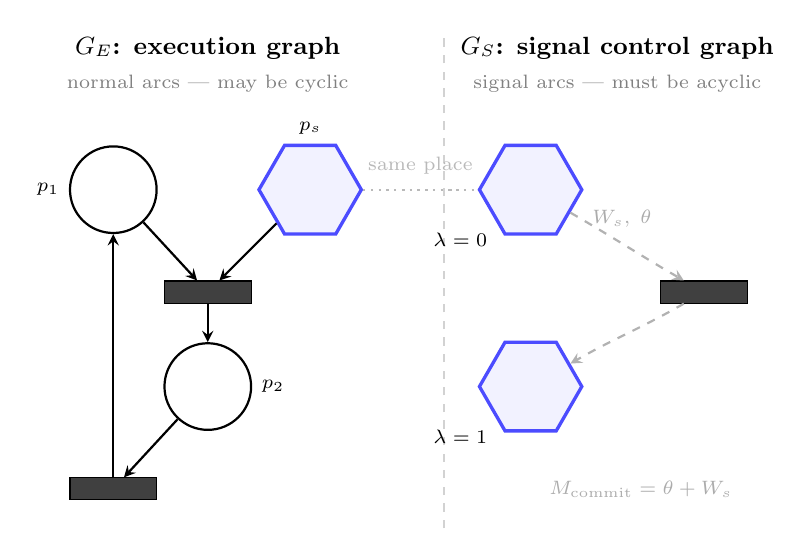
\begin{tikzpicture}[
  %% Normal place: black circle
  place/.style={circle, draw=black, thick, minimum size=1.1cm},
  %% Signal place: hexagon, blue border, very light blue fill
  sigplace/.style={regular polygon, regular polygon sides=6,
                   draw=blue!70, very thick, minimum size=1.3cm, fill=blue!5},
  %% Transition bar --- horizontal (flipped 90\textdegree)
  bar/.style={rectangle, draw=black, fill=black!75,
              minimum width=1.1cm, minimum height=0.28cm},
  %% Normal arc: black solid, 0.8pt
  arr/.style={->, >=stealth, line width=0.8pt},
  %% Signal arc: light gray dashed, 0.8pt
  sarr/.style={->, >=stealth, dashed, draw=gray!60, line width=0.8pt},
  every label/.style={font=\scriptsize}
]

%% ---- LEFT PANEL: G_E (execution graph) ----
\node[font=\small\bfseries] at (1.7, 6.1) {$G_E$: execution graph};
\node[font=\scriptsize, text=gray, align=center] at (1.7, 5.65)
     {normal arcs --- may be cyclic};

\node[place,    label={[font=\scriptsize]left:$p_1$}]   (p1) at (0.5, 4.3) {};
\node[sigplace, label={[font=\scriptsize]above:$p_s$}]  (ps) at (3.0, 4.3) {};
\node[bar]                                               (t1) at (1.7, 3.0) {};
\node[place,    label={[font=\scriptsize]right:$p_2$}]  (p2) at (1.7, 1.8) {};
\node[bar]                                               (t2) at (0.5, 0.5) {};

\draw[arr] (p1)       -- (t1);
\draw[arr] (ps)       -- (t1);
\draw[arr] (t1)       -- (p2);
\draw[arr] (p2) -- (t2);
\draw[arr] (t2) -- (p1);

%% ---- DIVIDER ----
\draw[dashed, gray!35, thick] (4.7, 0.0) -- (4.7, 6.3);

%% ---- RIGHT PANEL: G_S (signal control graph) ----
\node[font=\small\bfseries] at (6.9, 6.1) {$G_S$: signal control graph};
\node[font=\scriptsize, text=gray, align=center] at (6.9, 5.65)
     {signal arcs --- must be acyclic};

\node[sigplace, label={[font=\scriptsize]below left:$\lambda=0$}] (ps0) at (5.8, 4.3) {};
\node[sigplace, label={[font=\scriptsize]below left:$\lambda=1$}] (ps1) at (5.8, 1.8) {};
\node[bar]                                                         (tc)  at (8.0, 3.0) {};

\draw[sarr] (ps0) to[out=330, in=150]
     node[above=2pt, font=\scriptsize, text=gray!65, pos=0.45] {$W_s,\;\theta$}
     (tc);
\draw[sarr] (tc) to[out=210, in=30]
     (ps1);

\node[font=\scriptsize, text=gray!65, align=center] at (7.2, 0.5)
     {$M_{\mathrm{commit}} = \theta + W_s$};

%% ---- BRIDGE: same signal place in both panels ----
\draw[dotted, line width=0.8pt, gray!55] (ps.east) to[out=0, in=180]
     node[above=2pt, font=\scriptsize, pos=0.5] {same place}
     (ps0.west);

\end{tikzpicture}
\caption{\textbf{\DIFaddFL{Dual-graph architecture of SHPN.}} \DIFaddFL{The execution graph $G_E$
(left) carries stoichiometric mass transfer through normal arcs (solid black)
and may contain cycles. Signal places (blue hexagons, $p_s$) participate in
both graphs simultaneously. The signal control graph $G_S = (\Psi, F_s)$
(right) extracts those places into a directed acyclic graph (POSet); dashed
arcs carry signal weight $W_s$ and basin-floor threshold $\theta$, giving the
commitment criterion $M_{\mathrm{commit}} = \theta + W_s$. Layer depth
$\lambda$ encodes the hierarchy of commitment decisions. Acyclicity of $G_S$
formalizes biological irreversibility: a committed cell cannot uncommit through
the same hierarchical channel. Cycles in $G_E$ remain fully unrestricted.}}
\label{fig:dual_graph}
\end{figure}

\DIFaddend % Theory Section - Signal Hierarchy Theory
\section{Signal Hierarchy Theory}

We establish formal foundations for hierarchical biological control systems by proving structural properties of signal flow networks \cite{petri1962,murata1989}. The theory introduces three conceptual innovations enabling threshold predictability: (1) signal flow graphs as directed acyclic graphs enforcing hierarchical organization, (2) preemption semantics where lower-layer depletion disables higher-layer transitions, and (3) basin boundaries computable from network topology without simulation.

\subsection{Fundamental Concepts}

\begin{definition}[Signal Flow Graph]
\DIFaddbegin \DIFadd{Let $T$ be the set of transitions of the underlying Petri net. }\DIFaddend A signal flow graph \DIFdelbegin \DIFdel{$G_s = (\Psi, E_s)$ }\DIFdelend \DIFaddbegin \DIFadd{$G_s = (\Psi, F_s)$ }\DIFaddend consists of signal places \DIFdelbegin \DIFdel{$\Psi$ }\DIFdelend \DIFaddbegin \DIFadd{$\Psi \subseteq P$ }\DIFaddend (information channels) and signal flow \DIFdelbegin \DIFdel{edges $E_s \subseteq (\Psi \times T) \cup (T \times \Psi)$ }\DIFdelend \DIFaddbegin \DIFadd{arcs $F_s \subseteq (\Psi \times T) \cup (T \times \Psi)$ }\DIFaddend representing consumptive information propagation. Unlike metabolic arcs transferring mass, signal flow arcs transfer regulatory information consumed during transition firing.
\end{definition}

\begin{definition}[Layer Function]
A layer function $\lambda: \Psi \rightarrow \mathbb{N}_0$ assigns hierarchical depth to signal places via topological sort of $G_s$. For all signal flow edges, we enforce:
\begin{align*}
(p_i,t) \in F_s \wedge (t,p_j) \in F_s &\implies \lambda(p_i) < \lambda(p_j)
\end{align*}
establishing directed information flow from lower (metabolic) to higher (regulatory) layers.
\end{definition}

\begin{definition}[Basin Boundary]
For transition $t$ with signal input arc $(p_s,t) \in F_s$, the commitment marking
\begin{equation*}
M_{\text{commit}}(p_s) = \theta(t) + W_s((p_s,t))
\end{equation*}
defines basin boundary partitioning reachable state space:
\begin{itemize}
\item \textbf{Below boundary:} $B_{\text{below}} = \{M : M(p_s) < M_{\text{commit}}(p_s)\}$ (transition $t$ disabled)
\item \textbf{At boundary:} $B_{\text{boundary}} = \{M : M(p_s) = M_{\text{commit}}(p_s)\}$ (firing consumes $W_s$, leaves residual $M'(p_s) = \theta(t)$)
\item \textbf{Above boundary:} $B_{\text{above}} = \{M : M(p_s) > M_{\text{commit}}(p_s)\}$ (firing optional)
\end{itemize}
Firing from $M \in B_{\text{boundary}}$ produces $M' \in B_{\text{below}} \cup B_{\text{boundary}}$ when
$M'(p_s) = \theta(t) \leq M_{\text{commit}}(p_s)$,
creating one-way barrier: no firing sequence from $B_{\text{below}}$ reaches $B_{\text{above}}$ after signal consumption.
\end{definition}

\subsection{Structural Theorems}

\begin{theorem}[Acyclicity Requirement]
Signal flow graphs must be directed acyclic graphs (DAGs). Formally: \DIFdelbegin \DIFdel{$G_s = (\Psi, E_s)$ }\DIFdelend \DIFaddbegin \DIFadd{$G_s = (\Psi, F_s)$ }\DIFaddend admits valid layer function
$\lambda: \Psi \rightarrow \mathbb{N}_0$
satisfying $\lambda(p_i) < \lambda(p_j)$ for all paths $p_i \xrightarrow{t} p_j$ if and only if $G_s$ is acyclic.
\end{theorem}

\begin{proof}
($\Rightarrow$) Assume valid layer function $\lambda$ exists satisfying $\lambda(p_i) < \lambda(p_j)$ for all edges $(p_i,t,p_j)$ where $t$ connects $p_i$ to $p_j$ via signal flow arcs. Suppose for contradiction that $G_s$ contains cycle
\[
p_1 \xrightarrow{t_1} p_2 \xrightarrow{t_2} \cdots \xrightarrow{t_n} p_1.
\]
By layer function constraint applied to each edge:
\begin{equation*}
\lambda(p_1) < \lambda(p_2) < \lambda(p_3) < \cdots < \lambda(p_n) < \lambda(p_1)
\end{equation*}
Combining inequalities yields $\lambda(p_1) < \lambda(p_1)$, contradicting irreflexivity of $<$ on $\mathbb{N}_0$. Therefore $G_s$ must be acyclic.

($\Leftarrow$) Assume $G_s$ is acyclic. We construct valid $\lambda$ via topological sort algorithm:
\begin{enumerate}
\item Initialize $\lambda(p) = 0$ for all $p \in \Psi$
\item While exist unprocessed places: select $p$ with indegree 0 in remaining graph
\item For each outgoing edge $(p,t,p')$: set $\lambda(p') = \max(\lambda(p'), \lambda(p) + 1)$
\item Remove $p$ from graph, update indegrees
\end{enumerate}
Algorithm terminates because $G_s$ is finite and acyclic (no place depends on itself). For any edge $(p_i,t,p_j)$, topological ordering ensures $p_i$ processed before $p_j$, thus
$\lambda(p_i) < \lambda(p_j)$
by construction. Hence valid layer function exists.
\end{proof}

\textbf{Biological significance:} Acyclicity ensures commitment finality---once a decision is made through connected hierarchical channels, there is no alternative path back. When a cell commits to sporulation by consuming \DIFdelbegin \DIFdel{ATP signal through $(ATP, t_{\text{commit}}) \in F_s$, it }\DIFdelend \DIFaddbegin \DIFadd{$\sigma_H$ through $(\sigma_H, T_{\text{septation}}) \in F_s$---crossing the $\theta_{\sigma H} = 1.60\,\mu$M separatrix---it }\DIFaddend must follow that biochemical program irreversibly. The cell cannot "uncommit" and return to vegetative growth through the same signal flow path that triggered commitment. However, feedback regulation occurs abundantly through remote sensing: transcription factors can sense metabolite concentrations via rate functions $\Phi$ without creating reversible commitment paths. The acyclicity constraint applies to topology-explicit connected paths (signal flow arcs $F_s$ defining irreversible commitment structure), not to equation-implicit remote observations (rate functions $\Phi$ enabling feedback without reversibility). Signal consumption creates one-way state transitions: firing from basin boundary $M_{commit}$ depletes signals, making reverse traversal impossible. This formalizes biological commitment: development proceeds forward through irreversible decisions, while metabolic feedback maintains homeostasis through remote sensing.

\begin{theorem}[Hierarchical Preemption]
Lower-layer signal depletion structurally disables higher-layer transitions\DIFaddbegin \DIFadd{,
assuming the PreemptionCheck predicate is enforced: transition $t_j$ is enabled
only if every transition $t_i$ that produces its signal inputs via $F_s$ paths
is itself enabled}\DIFaddend .
Formally: if $\lambda(p_i) < \lambda(p_j)$ and there exists connected path $p_i \rightsquigarrow p_j$ through signal flow arcs, then
\[
M(p_i) < \theta(t_i) \text{ for any } t_i \in {}^\bullet p_j \implies \neg\text{Enabled}(t_j, M) \text{ for all } t_j \in p_j^\bullet,
\]
regardless of $M(p_j)$.
\end{theorem}

\begin{proof}
We prove by induction on layer depth $k = \lambda(p_j) - \lambda(p_i)$.

\textbf{Base case} ($k=1$): Places $p_i, p_j$ in adjacent layers with $\lambda(p_i) = \ell$ and $\lambda(p_j) = \ell+1$. By layer function definition, there exists $(p_i,t_i) \in F_s$ and $(t_i,p_j) \in F_s$. Signal enablement requires
$M(p_i) \geq \theta(t_i) + W_s((p_i,t_i))$
(by SignalEnabled predicate). If $M(p_i) < \theta(t_i)$, then
$M(p_i) < \theta(t_i) + W_s((p_i,t_i))$,
hence $\neg\text{SignalEnabled}(t_i,M)$, thus $\neg\text{Enabled}(t_i,M)$. Therefore $t_i$ cannot fire, preventing production of $p_j$ tokens. For any $t_j \in p_j^\bullet$, the PreemptionCheck$(t_j,M)$ requires Enabled$(t_i,M)$, which is false. Hence $\neg\text{Enabled}(t_j,M)$.

\textbf{Inductive step}: Assume true for all layer gaps $k' < k$. Consider $p_i, p_j$ with $\lambda(p_j) - \lambda(p_i) = k > 1$. There exists intermediate place $p_m$ with $\lambda(p_i) < \lambda(p_m) < \lambda(p_j)$ on path $p_i \rightsquigarrow p_m \rightsquigarrow p_j$. By inductive hypothesis applied to $(p_i,p_m)$ with gap $\lambda(p_m) - \lambda(p_i) < k$: if $M(p_i) < \theta(t_i)$, then all transitions producing $p_m$ are disabled, preventing $p_m$ production. Applying inductive hypothesis to $(p_m,p_j)$ with gap $\lambda(p_j) - \lambda(p_m) < k$: disabled transitions at $p_m$ prevent $p_j$ production, thus disabling all $t_j \in p_j^\bullet$. Transitive closure over path completes proof.
\end{proof}

\textbf{Biological significance:} \DIFdelbegin \DIFdel{ATP depletion below threshold disables sporulation regardless of sigma factor }\DIFdelend \DIFaddbegin \DIFadd{$\sigma_H$ depletion below the commitment separatrix ($\theta_{\sigma H} = 1.60\,\mu$M) structurally disables septation and all downstream execution layers, regardless of Spo0A$\sim$P }\DIFaddend abundance. A cell with saturating \DIFdelbegin \DIFdel{$\sigma^F$ but insufficient ATP cannot commit---energy constraint overrides regulatory }\DIFdelend \DIFaddbegin \DIFadd{phosphorelay output but $\sigma_H$ below threshold cannot commit---the commitment gate overrides integration-layer }\DIFaddend readiness. This captures \DIFdelbegin \DIFdel{metabolic override: lower metabolic layers veto higher regulatory layers }\DIFdelend \DIFaddbegin \DIFadd{hierarchical override: Layer~2 preempts Layer~3 }\DIFaddend through threshold enforcement, preventing \DIFdelbegin \DIFdel{energetically infeasible commitments}\DIFdelend \DIFaddbegin \DIFadd{commitment without the required $\sigma_H$ signal}\DIFaddend .

\subsection{Basin Boundary Computability}

\begin{theorem}[Irreversible Basin Partition]
For signal place $p_s \in \Psi$ with signal flow arc $(p_s,t) \in F_s$,
\DIFaddbegin \DIFadd{assuming no other transition regenerates $p_s$ via $F_s$ (i.e., there is no
$t' \neq t$ with $(t',p_s) \in F_s$), }\DIFaddend firing transition $t$ from commitment
marking $M_{\text{commit}}(p_s) = \theta(t) + W_s((p_s,t))$ creates \DIFaddbegin \DIFadd{a }\DIFaddend one-way
barrier in \DIFaddbegin \DIFadd{the }\DIFaddend reachability graph. Formally, let:
\begin{align*}
B_{\text{above}} &= \{M \in \mathcal{R}(M_0) : M(p_s) > M_{\text{commit}}(p_s)\} \\
B_{\text{boundary}} &= \{M \in \mathcal{R}(M_0) : M(p_s) = M_{\text{commit}}(p_s)\} \\
B_{\text{below}} &= \{M \in \mathcal{R}(M_0) : M(p_s) < M_{\text{commit}}(p_s)\}
\end{align*}
where $\mathcal{R}(M_0)$ denotes reachable markings. Then firing $t$ from any $M \in B_{\text{boundary}}$ produces $M' \in B_{\text{below}} \cup B_{\text{boundary}}$, and no firing sequence from $B_{\text{below}}$ produces \DIFaddbegin \DIFadd{a }\DIFaddend marking in $B_{\text{above}}$\DIFdelbegin \DIFdel{when signal consumption prevents $p_s$ regeneration}\DIFdelend .
\end{theorem}

\begin{proof}
Consider marking $M \in B_{\text{boundary}}$ with
$M(p_s) = M_{\text{commit}}(p_s) = \theta(t) + W_s((p_s,t))$.
By signal enablement, $M(p_s) \geq \theta(t) + W_s((p_s,t))$ holds with equality. Firing $t$ consumes $W_s((p_s,t))$ tokens from $p_s$ (by firing rule for signal places), producing:
\begin{align*}
M'(p_s) &= M(p_s) - W_s((p_s,t)) + W_s((t,p_s)) \\
&= (\theta(t) + W_s((p_s,t))) - W_s((p_s,t)) + W_s((t,p_s)) \\
&= \theta(t) + W_s((t,p_s))
\end{align*}

If $W_s((t,p_s)) = 0$ (no backward signal flow), then
$M'(p_s) = \theta(t) < M_{\text{commit}}(p_s)$,
placing $M' \in B_{\text{below}}$.

For irreversibility, consider any $M \in B_{\text{below}}$ with $M(p_s) < M_{\text{commit}}(p_s)$. To reach $B_{\text{above}}$, must increase $M(p_s)$ by producing tokens through some transition $t'$ with $(t',p_s) \in F_s$. \DIFdelbegin \DIFdel{However, }\DIFdelend \DIFaddbegin \DIFadd{By hypothesis, no such }\DIFaddend $t'$ \DIFdelbegin \DIFdel{requires its own signal inputs satisfy thresholds. If $p_s$ is unique signal place (as in commitment scenarios), no other transition can produce $p_s$ tokens from $B_{\text{below}}$ when signal consumption has depleted the commitment quota}\DIFdelend \DIFaddbegin \DIFadd{exists}\DIFaddend . Thus $B_{\text{below}}$ \DIFdelbegin \DIFdel{becomes absorbing setunder commitment dynamics}\DIFdelend \DIFaddbegin \DIFadd{is an absorbing set: once below the commitment threshold, no reachable firing sequence returns to $B_{\text{above}}$}\DIFaddend .
\end{proof}

\begin{corollary}[Threshold Predictability]
Commitment thresholds are computable from network topology without simulation:
\[
M_{\text{commit}}(p_s) = \theta(t) + W_s((p_s,t))
\]
where $\theta(t)$ and $W_s$ derive from biological rate constants and stoichiometry.
\end{corollary}

\begin{proof}
Direct consequence of Basin Boundary Definition. The commitment marking $M_{\text{commit}}(p_s)$ is defined as the minimal marking enabling transition $t$ such that firing consumes exactly the decision quota, leaving residual $M'(p_s) = \theta(t)$ (the enablement threshold). By signal enablement condition SignalEnabled$(t,M)$:
\begin{equation*}
M(p_s) \geq \theta(t) + W_s((p_s,t)) \iff M(p_s) \geq M_{\text{commit}}(p_s)
\end{equation*}
The minimal such marking is
$M_{\text{commit}}(p_s) = \theta(t) + W_s((p_s,t))$
obtained by taking equality. Both parameters are formalism specifications: $\theta(t)$ is assigned via threshold function $\theta: T \rightarrow \mathbb{R}^{\geq 0}$, and $W_s((p_s,t))$ via signal weight function $W_s: F_s \rightarrow \mathbb{R}^+$. No simulation or state space exploration required---values obtained directly from model specification via arithmetic.
\end{proof}

This establishes threshold prediction as \textit{structural property} of signal hierarchical networks. Unlike parameter fitting requiring experimental data, topology-based computation proceeds from formalism alone: identify signal input arc $(p_s,t)$, extract threshold $\theta(t)$ and weight $W_s((p_s,t))$, compute commitment marking. Below $M_{\text{commit}}$, transitions remain disabled; above, firing becomes possible but non-mandatory; at boundary, firing creates irreversibility.

% Control Section - Signal Hierarchical Control
\section{Signal Hierarchical Control}

Signal hierarchical control introduces a \textit{graph of information} layered over the \textit{graph of execution}. The execution graph $(P, T, F)$ models biochemical transformations through ordinary places, transitions, and arcs following mass-action dynamics. The information graph $(\Psi, F_s)$ models regulatory architecture through signal places and signal flow arcs defining hierarchical dependencies. By assigning signal type to selected places and arcs, we create vertical information channels broadcasting mass availability from Layer 0 to higher regulatory layers, while horizontal execution proceeds through stoichiometric transformations. This dual-graph architecture enables formal specification of control mechanisms: layer functions assign hierarchical organization, enablement predicates formalize vertical dependencies, signal consumption creates commitment semantics, and preemption mechanisms enforce irreversible decisions through state space partitioning.

\subsection{Signal Consumption Semantics}

The information graph operates through consumptive signal semantics distinct from classical arc types. Signal flow arcs $F_s$ implement information propagation where token consumption at Layer $k$ triggers enablement re-evaluation at layers $\ell > k$. This differs from:

\textbf{Normal arcs} ($F$): Model horizontal mass transfer with stoichiometric conservation. Firing consumes $W((p,t))$ inputs, produces $W((t,p))$ outputs, preserving molecular species through Layer 0 transformations.

\textbf{Test arcs} ($F_t$): Model catalysis through non-consuming local observation. Require $M(p) \geq W_t((p,t))$ without token transfer, enabling rate acceleration via arc-connected catalysts.

\textbf{Signal flow arcs} ($F_s$): Model vertical information broadcast with consumptive commitment. These arcs require marking
$M(p_s) \geq \theta(t) + W_s((p_s,t))$
and consume decision quota $W_s((p_s,t))$ upon firing. Unlike horizontal mass conservation (normal arcs) or local catalysis (test arcs), signal consumption creates irreversibility---tokens represent commitment resources depleted upon firing, establishing one-way state transitions partitioning reachability space. The arc semantics
$M'(p_s) = M(p_s) - W_s((p_s,t)) + W_s((t,p_s))$
couple token transfer with vertical broadcast to all layers $\ell > \lambda(p_s)$.

The information graph thus layers hierarchical control over biochemical execution: signal places serve as interfaces where Layer 0 mass dynamics broadcast regulatory information vertically through consumptive arcs, while horizontal transformations proceed through conserved mass transfer.

%DIF >  [R2-Phi] Remote sensing / rate functions Phi:
%DIF >  R2 argues Phi subsumes everything (any function of any place = any formalism).
%DIF >  The current text does not explain: (1) what Phi is restricted to reading,
%DIF >  (2) why Phi does not make signal flow arcs redundant,
%DIF >  (3) how Phi is actually used in the case study.
%DIF >  Fix: add a paragraph scoping Phi -- what it may read (topology-reachable places
%DIF >  or designated signal places), why the structural constraint is on G_S topology
%DIF >  not on the rate expression, and a concrete usage example.
\subsection{Connected vs. Remote Information Access}

The formalism distinguishes between topology-explicit (connected) and equation-implicit (remote) concentration information transfer:

\textbf{Connected channels (Signal flow arcs $F_s$):} Created by assigning type ``signal'' to normal arcs, coupling horizontal mass transfer with vertical information broadcast. Signal flow arcs $F_s$ are ordinary arcs $(p_s, t) \in F$ to which we assign signal semantics: token transfer at Layer $k$ (horizontal mass flow) triggers enablement re-evaluation at layers $\ell > k$ (vertical information broadcast). Signal places $p_s \in \Psi$ function as information hubs through this type assignment: the same places receive mass via metabolic reactions (normal arcs $F$) and broadcast availability via signal flow arcs $F_s$. This creates an interface from Layer 0 (executive metabolic layer) to higher regulatory layers---mass flows horizontally through biochemical transformations, information about mass availability broadcasts vertically to the cellular regulatory environment. Arc topology makes regulatory dependencies explicit---connected paths define hierarchical control flow.

\textbf{Remote sensing (Rate functions $\Phi$):} Implement mathematical dependencies where transitions reference places outside arc-connected locality. A transition $t$ can sense $M(p_{\text{remote}})$ without any arc
$(p_{\text{remote}}, t) \in F \cup F_s \cup F_t$
connecting them. This enables distance-independent regulation through kinetic equations
$\Phi(t) = f(M(p_1), M(p_2), \ldots, M(p_{\text{remote}}))$
where places $p_{\text{remote}}$ may be topologically distant. Remote sensing operates through equation-implicit references without token transfer.
\DIFaddbegin \DIFadd{Critically, the remote-sensed place $p_{\text{remote}}$ need not belong to $\Psi$, need not carry any $F_s$ arc, and need not participate in the commitment path in any way. A Layer-3 execution sigma factor can sense a Layer-0 metabolite via $\Phi$ (feedback inhibition); a metabolic rate can depend on a downstream product (end-product inhibition); any place in $P$ may appear in any rate function. Because $\Phi$ creates no $F_s$ arc, none of these dependencies appear in $G_S$ and none can create a preemption cycle. The acyclicity constraint governs only $G_S$ topology; $\Phi$ is completely unrestricted in its read set.
Table~\ref{tab:connected_remote} summarises the key differences between the two access modes.
}\DIFaddend 

\begin{table}[h]
\centering
\footnotesize
\caption{Connected vs. Remote Information Propagation}
\DIFaddbeginFL \label{tab:connected_remote}
\DIFaddendFL \begin{tabular}{p{2.2cm}p{3.9cm}p{3.9cm}}
\toprule
\textbf{Property} & \textbf{Connected ($F_s$)} & \textbf{Remote ($\Phi$)} \\
\midrule
Mechanism & Physical arc & Mathematical dependency \\
Topology & Explicit in graph & Implicit in equations \\
Token transfer & Consumptive: $M' = M - W_s$ & Observational only \\
Locality & Direct connection & Any place \\
Vertical flow & Yes (layers $\ell > k$) & No (local only) \\
Preemption & Hierarchical disabling & No hierarchical effect \\
Reversibility & Irreversible & Reversible \\
Example & \DIFdelbeginFL \DIFdelFL{ATP $\xrightarrow{F_s}$ KinA }\DIFdelendFL \DIFaddbeginFL \DIFaddFL{$\sigma_H \xrightarrow{F_s} T_{\text{septation}}$ }\DIFaddendFL & \DIFdelbeginFL \DIFdelFL{TF }\DIFdelendFL \DIFaddbeginFL \DIFaddFL{Spo0A$\sim$P }\DIFaddendFL sensing via $\Phi$ \\
\bottomrule
\end{tabular}
\end{table}

Test arcs $F_t$ implement non-consumptive observation of arc-connected places (local catalysis), distinct from remote sensing which operates through rate function global references without physical connection. Both connected channels and remote sensing provide concentration information: connected channels couple consumption with hierarchical broadcast through explicit topology for irreversible commitment, while remote sensing enables distance-independent regulation preserving local topology without preemption influence.

\DIFaddbegin \textbf{\DIFadd{Remark ($\Phi$ and $F_s$ serve structurally distinct roles):}} \DIFadd{Rate functions $\Phi$ are inherited unchanged from standard Bio-PN. A natural question is whether $\Phi$, being able to encode any function of any state variable, makes $F_s$ redundant. It does not: $\Phi$ operates over $G_E$---modelling continuous, reversible kinetics whose read dependencies may be cyclic---while $F_s$ operates over $G_S$---modelling discrete, irreversible commitment whose topology must be acyclic. The structural theorems (Acyclicity, Preemption, Basin Partition) are properties of $G_S$: they cannot be recovered from rate functions alone because $\Phi$ is not subject to the DAG constraint that makes them provable. In the limit---a net with all regulation in $\Phi$ and no arcs---the marking never changes from $M_0$ and there is no basin boundary. The moment you add a signal flow arc you get an irreversible commitment boundary with threshold $M_{\text{commit}} = \theta + W_s$. $\Phi$ expresses what a transition }\textit{\DIFadd{reads}}\DIFadd{; only $F_s$ arcs determine what it }\textit{\DIFadd{destroys}}\DIFadd{, and it is destruction that makes commitment irreversible.
}

\DIFaddend \subsection{Hierarchical Enablement}

\begin{definition}[Hierarchical Enablement Predicate]
Transition $t$ is hierarchically enabled at marking $M$ if:
\begin{align}
\text{Enabled}(t, M) &\equiv \text{NormalEnabled}(t,M) \nonumber \\
&\wedge \text{TestEnabled}(t,M) \nonumber \\
&\wedge \text{SignalEnabled}(t,M) \nonumber \\
&\wedge \text{PreemptionCheck}(t,M)
\end{align}
\end{definition}

where we define notation:
\begin{itemize}
\item ${}^\bullet t = \{p \in P : (p,t) \in F\}$ (normal input places)
\item $t^\bullet = \{p \in P : (t,p) \in F\}$ (normal output places)
\item ${}^\bullet_s t = \{p_s \in \Psi : (p_s,t) \in F_s\}$ (signal input places)
\item $t^\bullet_s = \{p_s \in \Psi : (t,p_s) \in F_s\}$ (signal output places)
\item ${}^\bullet_s p = \{t \in T : (t,p) \in F_s\}$ (transitions producing place via signal arcs)
\item $p^\bullet_s = \{t \in T : (p,t) \in F_s\}$ (transitions consuming place via signal arcs)
\item $\text{Test}(t) = \{p \in P : (p,t) \in F_t\}$ (test arc places)
\end{itemize}

and predicates:
\begin{align}
\text{NormalEnabled}(t,M) &\equiv \forall p \in {}^\bullet t: M(p) \geq W((p,t)) \\
\text{TestEnabled}(t,M) &\equiv \forall p \in \text{Test}(t): M(p) \geq \tau_t((p,t)) \\
\text{SignalEnabled}(t,M) &\equiv \forall p_s \in {}^\bullet_s t: M(p_s) \geq \theta(t) + W_s((p_s,t)) \\
\text{PreemptionCheck}(t,M) &\equiv \forall p_s \in {}^\bullet_s t: \forall t' \in {}^{\bullet}_s p_s: \nonumber \\
&\quad (\text{NormalEnabled}(t',M) \wedge \text{TestEnabled}(t',M) \nonumber \\
&\quad \wedge \text{SignalEnabled}(t',M))
\end{align}

The PreemptionCheck enforces hierarchical dependencies by requiring all transitions producing input signal places (via signal flow arcs) satisfy their local enablement conditions. This is a \textit{single-layer} check: only immediate signal-producing predecessors are verified, not transitive ancestors. Hierarchical consistency propagates automatically because each layer's PreemptionCheck verifies its direct predecessors, creating cascading verification back to Layer 0 through the acyclic structure.

\subsection{Firing Rule}

\begin{definition}[Firing Function]
Upon firing enabled transition $t$ at marking $M$, the firing function $\text{Fire}(t,M)$ produces new marking $M'$ where:
\begin{equation}
M'(p) = M(p) + \Delta_{\text{normal}}(p,t) + \Delta_{\text{signal}}(p,t)
\end{equation}
with token changes:
\begin{align}
\Delta_{\text{normal}}(p,t) &= \begin{cases}
-W((p,t)) + W((t,p)) & \text{if } (p,t) \in F \text{ or } (t,p) \in F \\
0 & \text{otherwise}
\end{cases} \\
\Delta_{\text{signal}}(p,t) &= \begin{cases}
-W_s((p,t)) + W_s((t,p)) & \text{if } (p,t) \in F_s \text{ or } (t,p) \in F_s \\
0 & \text{otherwise}
\end{cases}
\end{align}
\end{definition}

Test arcs do not affect marking: $(p,t) \in F_t$ implies $M'(p) = M(p)$ (non-consuming observation).

\textbf{Remark (sensing threshold vs.\ kinetic weight):} The predicate $\text{TestEnabled}$ uses the \emph{sensing threshold} $\tau_t((p,t)) \geq 0$, which is distinct from the \emph{kinetic weight} $W_t((p,t))$ appearing in the rate function $\Phi(t)$. $\tau_t$ encodes the activation level of the local wired sensor---the minimum signal required to declare the transition enabled---while $W_t$ is a kinetic modulation parameter (e.g., $K_m$ in a Michaelis-Menten term). These quantities have different scaling laws: when initial conditions are rescaled by factor $\alpha$, explicitly-set $\tau_t > 0$ must scale by $\alpha$ to preserve enablement semantics, while $W_t$ (an intensive parameter embedded in $\Phi$) is unchanged. The default $\tau_t = 0$ implements a pure \emph{presence check} ($M(p) > 0$), which is scale-invariant and biologically appropriate when catalytic action requires only that the species be present.

\textbf{Dual arc case:} When $p \in \Psi$ with both $(p,t) \in F$ and $(p,t) \in F_s$, firing consumes tokens from both normal and signal weights: $M'(p) = M(p) - W((p,t)) - W_s((p,t)) + W((t,p)) + W_s((t,p))$.

Signal consumption depletes regulatory tokens, creating state space partitions: markings below commitment threshold cannot reach markings above after firing.

\subsection{Layer Assignment Algorithm}

\begin{algorithm}
\caption{Hierarchical Layer Assignment}
\begin{algorithmic}[1]
\Require Signal flow graph \DIFdelbegin \DIFdel{$G_s = (\Psi, E_s)$ where $E_s = F_s \cap ((\Psi \times T) \cup (T \times \Psi))$
}\DIFdelend \DIFaddbegin \DIFadd{$G_s = (\Psi, F_s)$
}\DIFaddend \Ensure Layer function $\lambda: \Psi \rightarrow \mathbb{N}_0$ or FAIL if $G_s$ contains cycle
\State $\lambda(p) \leftarrow 0$ for all $p \in \Psi$
\State $\text{indeg}(p) \leftarrow |\{(p',t) \in F_s, (t,p) \in F_s\}|$ for all $p \in \Psi$ \Comment{Count incoming signal paths}
\State $Q \leftarrow \{p \in \Psi : \text{indeg}(p) = 0\}$ \Comment{Source signal places}
\State $\text{processed} \leftarrow 0$
\While{$Q \neq \emptyset$}
    \State $p \leftarrow Q.\text{dequeue}()$
    \State $\text{processed} \leftarrow \text{processed} + 1$
    \For{each $(p,t) \in F_s$ and $(t,p') \in F_s$} \Comment{Outgoing signal paths through $t$}
        \State $\lambda(p') \leftarrow \max(\lambda(p'), \lambda(p) + 1)$
        \State $\text{indeg}(p') \leftarrow \text{indeg}(p') - 1$
        \If{$\text{indeg}(p') = 0$}
            \State $Q.\text{enqueue}(p')$
        \EndIf
    \EndFor
\EndWhile
\If{$\text{processed} < |\Psi|$}
    \State \Return FAIL \Comment{Cycle detected}
\Else
    \State \Return $\lambda$
\EndIf
\end{algorithmic}
\end{algorithm}

\textbf{Complexity:} $O(|\Psi| + |F_s|)$ via modified topological sort. Algorithm fails if $G_s$ contains cycles, providing constructive verification of acyclicity theorem.

\subsection{Commitment Semantics}
\DIFaddbegin \label{sec:commitment_semantics}
\DIFaddend 

Commitment occurs when transition fires from basin boundary marking:
\begin{enumerate}
\item \textbf{Pre-commitment}: $M(p_s) < M_{\text{commit}}(p_s)$ --- transition disabled, cell uncommitted
\item \textbf{Commitment boundary}: $M(p_s) = M_{\text{commit}}(p_s)$ --- transition enabled, firing creates irreversibility
\item \textbf{Post-commitment}: $M(p_s) \geq M_{\text{commit}}(p_s)$ and fired --- residual marking $M'(p_s) = \theta(t)$ prevents return
\end{enumerate}

The key insight: signal consumption creates one-way transition. Unlike normal Petri nets where reverse firing can restore markings, signal depletion establishes state space partitioning---committed cells cannot uncommit through any firing sequence. Once a cell commits to sporulation by firing $t_{commit}$ from basin boundary, consuming signal tokens, there is no alternative biochemical path back to the vegetative state through the same connected hierarchy. The commitment becomes final---the cell must follow the sporulation program forward. This captures biological reality: developmental commitment proceeds irreversibly through forward-only paths, even though metabolic feedback loops maintain homeostasis through remote sensing mechanisms.

%DIF <  Formalism Section
\DIFaddbegin \begin{figure}[H]
    \centering
    
\includegraphics[width=\columnwidth]{figures/fig_preemption_cascade_v3.pdf}
    \caption{%DIF > 
        \textbf{\DIFaddFL{PreemptionCheck in action: stochastic commitment collapses to quasi-continuous execution.}}
        \DIFaddFL{Individual trajectories of three key cascade species across 50 stochastic $\tau$-leaping replicates
        of the }\textit{\DIFaddFL{B.~subtilis}} \DIFaddFL{sporulation model
        ($N_0 = 1440\,\mu$M, SinR $= 12\,\mu$M, run\_20260614\_123652).
        Red: sporulating replicates (24/50); grey: vegetative replicates (26/50). Thick lines: fate-conditioned means.
        }\textit{\DIFaddFL{Bottom}} \DIFaddFL{— Spo0A$\sim$P: stochastic phosphorelay; both fates share indistinguishable variance until $t_\mathrm{commit}$.
        }\textit{\DIFaddFL{Middle}} \DIFaddFL{— $\sigma_H$: commitment gate; violet dashed line marks $\theta_{\sigma H} = 1.60\,\mu$M; only sporulating replicates cross it.
        }\textit{\DIFaddFL{Top}} \DIFaddFL{— $\sigma_F$: execution programme; silent in vegetative replicates; activates post-commitment with markedly reduced variance, demonstrating the quasi-continuous character of execution once PreemptionCheck unlocks.
        The $\sigma_H$ separatrix is the basin boundary predicted analytically by the commitment semantics: once crossed, token consumption is irreversible and all downstream layers fire in lock-step.%DIF > 
    }}
    \label{fig:preemption_cascade}
\end{figure}

\DIFadd{The three-phase commitment semantics are directly observable in these trajectories (Fig~\ref{fig:preemption_cascade}).
Before $t \approx 240\,\mathrm{min}$ all 50 replicates are in the pre-commitment phase ($M(\sigma_H) < \theta_{\sigma H}$) and all downstream layers are structurally disabled by PreemptionCheck regardless of Spo0A$\sim$P abundance.
At $t_\mathrm{commit} = 300\,\mathrm{min}$ the stochastic $\sigma_H$ ramp crosses $\theta_{\sigma H}$ in a subset of replicates: these enter the commitment boundary and fire $T_{\mathrm{septation}}$, consuming signal tokens irreversibly.
Post-commitment, all downstream layers ($\sigma_F$, $\sigma_E$, $\sigma_G$, $\sigma_K$, forespore assembly) fire in near-deterministic sequence — the red fan in the top strip is visibly tighter than the phosphorelay fan below, quantifying the noise suppression imposed by hierarchical gating.
Replicates that never cross $\theta_{\sigma H}$ (grey) remain in the vegetative basin with $\sigma_F \equiv 0$ indefinitely: no alternative firing sequence can reach the sporulation attractor.
}\DIFaddend 

% Formalism Section
\DIFaddbegin \FloatBarrier
\DIFaddend \section{Signal Hierarchical Petri Nets}

We formalize signal hierarchical control as 13-tuple extension of classical Bio-PN, providing complete mathematical specification enabling computational implementation.

\subsection{Formal Definition}

\begin{definition}[Signal Hierarchical Petri Net]
A Signal Hierarchical Petri Net is a 13-tuple:
\begin{equation}
\text{SPN} = (P, T, F, W, M_0, \Phi, C, F_t, \Psi, F_s, W_s, \lambda, \theta)
\end{equation}
where:
\begin{itemize}
\item $(P, T, F, W, M_0)$ is classical 5-tuple (places, transitions, arcs, weights, initial marking)
\item $\Phi: T \rightarrow \text{RateFunctions}$ assigns kinetic rate laws to transitions
\item $C: F \rightarrow \text{Stoich}$ assigns stoichiometric coefficients to arcs
\item $F_t \subseteq P \times T$ defines test arcs (catalysis, non-consuming)\DIFaddbegin \DIFadd{; test arc enablement requires $M(p) \geq 1$ for all $(p,t) \in F_t$ --- the sensing threshold is uniformly~1 and is not a free parameter of the formalism
}\DIFaddend \item $\Psi \subseteq P$ defines signal places (information channels)
\item $F_s \subseteq (\Psi \times T) \cup (T \times \Psi)$ defines signal flow arcs
\item $W_s: F_s \rightarrow \mathbb{R}^+$ assigns signal arc weights
\item $\lambda: \Psi \rightarrow \mathbb{N}_0$ assigns hierarchical layers
\item $\theta: T \rightarrow \mathbb{R}^{\geq 0}$ assigns enablement thresholds
\end{itemize}
\end{definition}

\subsection{Architectural Principles}

\textbf{Vertical-Horizontal Separation:} Normal arcs $F$ model horizontal mass transfer (metabolic reactions), signal flow arcs $F_s$ model vertical information propagation (regulatory control). Signal places $p_s \in \Psi$ function as information hubs: metabolic transitions connect via normal arcs to modify $M(p_s)$ at Layer 0 (horizontal participation), while regulatory transitions connect via signal flow arcs to consume signals and broadcast state changes to higher layers (vertical participation). This architectural separation mirrors biological organization where metabolic networks operate horizontally through spatially-distributed enzyme cascades, while regulatory hierarchies operate vertically with metabolic state gating developmental decisions through connected signal paths.

\textbf{Connected vs. Remote Information Transfer:} The formalism provides two complementary mechanisms. Connected channels (signal flow arcs $F_s$) implement topology-explicit wired propagation where physical arc connections enable hierarchical preemption---consumption at layer $k$ triggers re-evaluation at all layers $\ell > k$. Remote sensing (rate functions $\Phi$) implements equation-implicit wireless observation where transitions reference concentrations of topologically distant places without physical connection---enabling long-range regulation through kinetic dependencies $\Phi(t) = f(M(p_{\text{remote}}))$ without hierarchical influence. Biologically, connected channels model committed resource allocation with hierarchical consequences (\DIFdelbegin \DIFdel{ATP consumption for sporulation entry disables downstream cascades}\DIFdelend \DIFaddbegin \DIFadd{$\sigma_H$ depletion below $\theta_{\sigma H} = 1.60\,\mu$M at commitment disables all downstream execution layers}\DIFaddend ), while remote sensing models long-range regulatory effects without physical transport (\DIFdelbegin \DIFdel{transcription factor }\DIFdelend \DIFaddbegin \DIFadd{Spo0A$\sim$P }\DIFaddend concentration influencing distant operon expression through equation dependencies).

\textbf{Dual Arc Semantics:} Signal places $p_s \in \Psi$ can simultaneously participate in both normal arcs (horizontal mass transfer) and signal flow arcs (vertical information propagation):
\begin{align}
\text{Normal arc}: &\quad (p_s, t) \in F \text{ with weight } W((p_s,t)) \in \mathbb{R}^+ \nonumber \\
&\quad \text{(stoichiometric consumption)} \\
\text{Signal arc}: &\quad (p_s, t) \in F_s \text{ with weight } W_s((p_s,t)) \in \mathbb{R}^+ \nonumber \\
&\quad \text{(regulatory quota)}
\end{align}

When transition $t$ fires with both arc types from place $p_s$, marking evolution is:
\begin{equation}
M'(p_s) = M(p_s) - W((p_s,t)) - W_s((p_s,t)) + W((t,p_s)) + W_s((t,p_s))
\end{equation}

This enables the same metabolite (e.g., ATP) to participate in biochemical reactions (glycolysis) and regulatory decisions (commitment gating) without duplication.

\DIFaddbegin \textbf{\DIFadd{Design principle --- selective wiretap on the physical layer:}} \DIFadd{Signal type assignment does not introduce new arcs, new places, or new tokens. It is a }\textit{\DIFadd{selective annotation}}\DIFadd{: the modeler designates certain existing normal arcs as signal flow arcs, so that the same token-consuming event that performs biochemistry in $G_E$ simultaneously reports a commitment to the control hierarchy $G_S$. The cell does not maintain two separate copies of a molecule---one for metabolism, one for signaling. There is one token; the type annotation gives its consumption a second, hierarchical meaning. This is why the two-graph architecture is necessary: $G_E$ must be free to cycle (metabolic feedback, oscillations, reversible reactions), while $G_S$ must be acyclic (commitments are one-way). The same token stream feeds both graphs; the arc type determines which graph records the event.
}

\DIFaddend \subsection{Operational Semantics}

\begin{definition}[Marking Evolution]
State space $\mathcal{M} = \mathbb{N}_0^{|P|}$ consists of all possible token distributions. Single-step reachability relation is:
\begin{equation}
M \xrightarrow{t} M' \iff \text{Enabled}(t, M) \wedge M' = \text{Fire}(t, M)
\end{equation}
Multi-step reachability $M \xrightarrow{*} M'$ is the reflexive transitive closure: $M \xrightarrow{*} M'$ holds if there exists firing sequence $t_1, t_2, \ldots, t_n$ with $M \xrightarrow{t_1} M_1 \xrightarrow{t_2} \cdots \xrightarrow{t_n} M'$ for some $n \geq 0$.
\end{definition}

\begin{definition}[Reachability Set]
The reachability set from initial marking $M_0$ is:
\begin{equation}
\mathcal{R}(M_0) = \{M \in \mathcal{M} : M_0 \xrightarrow{*} M\}
\end{equation}
Signal consumption creates reachability partition: $\mathcal{R}(M_0) = B_{\text{below}} \cup B_{\text{boundary}} \cup B_{\text{above}}$ where basin boundaries form one-way barriers (Theorem: Irreversible Basin Partition).
\end{definition}

\begin{proposition}[Hierarchical Decomposition]
For signal hierarchical PN with $k$ layers, reachability analysis decomposes into layer-wise subproblems. Analyzing Layer $\ell$ with fixed commitments from layers $0, \ldots, \ell-1$ reduces complexity from $O(\prod_{i=0}^{k} |M_{\text{Layer}_i}|)$ (product of layer state spaces) to $O(\sum_{i=0}^{k} |M_{\text{Layer}_i}| \cdot b_i)$ where $b_i$ is branching factor at layer $i$.
\end{proposition}

\begin{proof}
General reachability in Petri nets is EXPSPACE-complete \cite{esparza1996}, with state space exponential in number of places. For flat model with $\sum_i n_i$ places distributed across $k$ layers, reachability graph has $O(\prod_i C^{n_i})$ states where $C$ is token bound.

Hierarchical structure enables decomposition: (1) Analyze Layer 0 independently, computing commitment thresholds via $M_{\text{commit}} = \theta + W_s$ ($O(1)$ per transition). (2) Fix Layer 0 commitments, reducing Layer 1 to subproblem with Layer 0 constraints---state space now $O(C^{n_1} \cdot b_0)$ where $b_0$ bounds Layer 0 commitment states. (3) Repeat for layers $2, \ldots, k$.

Total complexity: sum over layers instead of product. For B. subtilis model (\DIFdelbegin \DIFdel{47 }\DIFdelend \DIFaddbegin \DIFadd{40 }\DIFaddend places, 4 layers): flat analysis requires \DIFdelbegin \DIFdel{$O(10^{47})$ }\DIFdelend \DIFaddbegin \DIFadd{$O(10^{40})$ }\DIFaddend states; hierarchical analysis requires \DIFdelbegin \DIFdel{$O(4 \cdot 10^{12})$ states---reduction of 35 }\DIFdelend \DIFaddbegin \DIFadd{$O(4 \cdot 10^{10})$ states---a reduction of 30 }\DIFaddend orders of magnitude \DIFaddbegin \DIFadd{that }\DIFaddend enables practical computation.
\end{proof}

\subsection{Comparison with Classical Bio-PN}

\DIFaddbegin \DIFadd{SHPN extends classical Bio-PN expressiveness through signal-type semantics, as summarised in Table~\ref{tab:comparison}.
}

\DIFaddend \begin{table}[h]
\centering
\small
\caption{Expressiveness Comparison: Classical Bio-PN vs. Signal Hierarchical PN}
\DIFaddbeginFL \label{tab:comparison}
\DIFaddendFL \begin{tabular}{p{5cm}p{2.5cm}p{2.5cm}}
\toprule
\textbf{Capability} & \textbf{Classical} & \textbf{Signal Hier.} \\
\midrule
Mass transfer & Yes & Yes \\
Catalysis (non-consuming) & Yes & Yes \\
Regulatory consumption & No & Yes \\
Hierarchical layers & No & Yes \\
Threshold semantics & No & Yes \\
Basin boundaries & No & Yes \\
Commitment irreversibility & No & Yes \\
Unified metabolic-regulatory & No & Yes \\
\DIFdelbeginFL \DIFdelFL{First-principles }\DIFdelendFL \DIFaddbeginFL \DIFaddFL{Topology-driven }\DIFaddendFL thresholds & No & Yes \\
\bottomrule
\end{tabular}
\end{table}

\textbf{Key distinction:} Test arcs enable transitions when $M(p) \geq W_t$ without token consumption, maintaining $M'(p) = M(p)$ after firing. Signal flow arcs require $M(p_s) \geq \theta + W_s$ and consume tokens, producing $M'(p_s) = M(p_s) - W_s$ after firing. This semantic difference between consumption and read-only behavior determines expressiveness: test arcs model catalysis such as enzyme-substrate binding, while signal flow arcs model commitment through decision quota depletion.

% Unified Modeling Section
\section{Unified Metabolic-Regulatory Modeling}

Signal hierarchical Petri nets enable integrated modeling where metabolic and regulatory networks share species through dual arc semantics. We demonstrate unified framework capability through multi-layer architecture.

\subsection{Signal Place Designation}

The formalism's power derives from modeler choice: any metabolite can be designated as signal place $p_s \in \Psi$ when biological evidence supports regulatory gating role. This designation determines dual participation through horizontal mass transfer and vertical information broadcast.

\vspace{3pt}
\noindent\textbf{Horizontal mass transfer.} Signal places are normal places participating in biochemical reactions via normal arcs $F$ at Layer 0. For example, ATP in glycolysis: $(t_{\text{glycolysis}}, \text{ATP}) \in F$ with $W = 2$ (stoichiometric production). NADH in oxidative phosphorylation: $(\text{NADH}, t_{\text{complex-I}}) \in F$ with $W = 1$ (consumption).

\vspace{3pt}
\noindent\textbf{Vertical information broadcast.} The same places, when we assign type ``signal,'' broadcast availability to higher regulatory layers via signal flow arcs $F_s$. For example, \DIFdelbegin \DIFdel{ATP signaling energy state: $(\text{ATP}, t_{\text{commit}}) \in F_s$ with $W_s = 0.17$ mM (commitment quota). GTP signaling translational capacity: $(\text{GTP}, t_{\text{transcribe}}) \in F_s$ with $W_s = 0.05$ mM (transcription quota}\DIFdelend \DIFaddbegin \DIFadd{$\sigma_H$ signaling commitment readiness: $(\sigma_H, T_{\text{septation}}) \in F_s$ with $W_s = \theta_{\sigma H} \approx 1.60\,\mu$M (commitment separatrix). Spo0A$\sim$P broadcasting phosphorelay output: $(\text{Spo0A}{\sim}\text{P},\, t_{\sigma H}) \in F_s$ (integration-to-commitment gating}\DIFaddend ).

This type assignment creates an interface from Layer 0 to higher layers: signal places and signal flow arcs are ordinary places and arcs to which we assign signal semantics, enabling the same places to participate in horizontal mass flow (metabolic transformations) and vertical information broadcast (regulatory propagation). Mass flows horizontally through stoichiometric reactions; information about mass availability broadcasts spatially (vertically) to the cellular regulatory environment. No artificial separation into distinct species---unified place, differentiated semantics through arc type assignment.

\textbf{Biological case selection:} For \textit{B. subtilis} sporulation, we designate \DIFdelbegin \DIFdel{ATP as primary signal place based on experimental evidence showing ATP-dependent commitment \mbox{%DIFAUXCMD
\cite{fujita2005}}\hskip0pt%DIFAUXCMD
. }\DIFdelend \DIFaddbegin \DIFadd{$\sigma_H$ as the commitment-gate signal place and Spo0A$\sim$P as the phosphorelay integration signal~\mbox{%DIFAUXCMD
\cite{fujita2005}}\hskip0pt%DIFAUXCMD
. ATP and GTP remain metabolic participants (via normal arcs) but are not the separatrix species: the commitment threshold is the $\sigma_H$ separatrix ($\theta_{\sigma H} = 1.60\,\mu$M), not an energy quota. }\DIFaddend Other systems designate different signals: calcium (Ca$^{2+}$) for neurotransmitter release, cyclic AMP (cAMP) for bacterial chemotaxis, GTP for protein synthesis quality control, NADH for metabolic oscillations. The formalism generalizes across signal types---designation derives from biological function, not molecular identity.

\subsection{Four-Layer Architecture with Multi-Level Signal Assignment}\DIFaddbegin \label{sec:four_layer}
\DIFaddend 

Signal places can be designated at \textit{any} hierarchical layer, not restricted to Layer 0. This design choice significantly enhances formalism expressiveness by enabling multi-stage commitment with cascading irreversibility. For the \textit{B. subtilis} case, signal places are \DIFdelbegin \DIFdel{strategically }\DIFdelend designated across all four layers \DIFaddbegin \DIFadd{as determined by the signal flow arc topology of the v9 model}\DIFaddend :

\vspace{3pt}
\noindent\textbf{Layer 0 (\DIFdelbegin \DIFdel{Metabolism}\DIFdelend \DIFaddbegin \DIFadd{Starvation Sensing}\DIFaddend ):} \DIFdelbegin \DIFdel{ATP, NADH designated as signals ($\lambda(\text{ATP}) = 0$). Normal arcs model glycolysis and TCA cycle producing metabolic signals}\DIFdelend \DIFaddbegin \DIFadd{KinA$_{\text{kinase}}$ designated as signal ($\lambda(\text{KinA}_{\text{kinase}}) = 0$). Rate $\propto \text{KinA}_{\text{kinase}} \cdot 1/(1+\text{Nutrients}^2)$: active only under starvation}\DIFaddend . Signal flow arcs \DIFdelbegin \DIFdel{broadcast metabolic state to Layer 1, creating }\DIFdelend \DIFaddbegin \DIFadd{connect KinA$_{\text{kinase}}$ to the phosphorelay entry, creating the }\DIFaddend first commitment barrier: \DIFdelbegin \DIFdel{insufficient ATP prevents sensing activation regardless of starvation signals}\DIFdelend \DIFaddbegin \DIFadd{absence of nutrient stress structurally disables all downstream layers regardless of phosphorylation state}\DIFaddend .

\vspace{3pt}
\noindent\textbf{Layer 1 (\DIFdelbegin \DIFdel{Sensing}\DIFdelend \DIFaddbegin \DIFadd{Phosphorelay Integration}\DIFaddend ):} \DIFdelbegin \DIFdel{CodY$_{\text{active}}$, CcpA$_{\text{active}}$ designated as signals ($\lambda(\text{CodY}) = 1$). Normal arcs model sensor activation. }\DIFdelend \DIFaddbegin \DIFadd{Spo0A$\sim$P designated as signal ($\lambda(\text{Spo0A}{\sim}\text{P}) = 1$). }\DIFaddend Signal flow arcs \DIFdelbegin \DIFdel{from Layer 0 metabolites enable sensing, while Layer 1 signals broadcast }\DIFdelend \DIFaddbegin \DIFadd{carry the phosphoryl group through the four-protein relay (KinA$_{\text{kinase}}$ $\to$ KinA$_{\text{P}}$ $\to$ Spo0F$_{\text{P}}$ $\to$ Spo0A$\sim$P), each step stochastic. Spo0A$\sim$P broadcasts }\DIFaddend to Layer 2, creating \DIFaddbegin \DIFadd{the }\DIFaddend second commitment barrier: \DIFdelbegin \DIFdel{sensor depletion preempts integration even if metabolites recover}\DIFdelend \DIFaddbegin \DIFadd{insufficient phosphorelay output prevents commitment-gate activation}\DIFaddend .

\vspace{3pt}
\noindent\textbf{Layer 2 (\DIFdelbegin \DIFdel{Integration}\DIFdelend \DIFaddbegin \DIFadd{Commitment Gate}\DIFaddend ):} \DIFdelbegin \DIFdel{Spo0A$\sim$P }\DIFdelend \DIFaddbegin \DIFadd{$\sigma_H$ }\DIFaddend designated as signal (\DIFdelbegin \DIFdel{$\lambda(\text{Spo0A}\sim\text{P}) = 2$). Normal arcs model phosphorelay (KinA-Spo0F-Spo0B-Spo0A). Signal flow arcs from Layer 1 sensors enable integration, while }\DIFdelend \DIFaddbegin \DIFadd{$\lambda(\sigma_H) = 2$). Produced by a Hill-4 positive-feedback switch on }\DIFaddend Spo0A$\sim$P \DIFdelbegin \DIFdel{signals to Layer 3, creating third commitment barrier: phosphorelay depletion prevents execution even if sensors remain active. }\DIFdelend \DIFaddbegin \DIFadd{($T_{\sigma H}$: $\Phi \propto \text{Spo0A}{\sim}\text{P}^4 / (50 + \text{Spo0A}{\sim}\text{P}^4)$); gates $T_{\text{septation}}$ rate as $\sigma_H^2$. The $\sigma_H$ separatrix $\theta_{\sigma H} = 1.60\,\mu$M is the analytically predicted commitment boundary: only replicates crossing it fire $T_{\text{septation}}$, consuming signal tokens irreversibly and unlocking Layer 3.
}\DIFaddend 

\vspace{3pt}
\noindent\textbf{Layer 3 (Execution):} $\sigma^F$, $\sigma^E$\DIFaddbegin \DIFadd{, $\sigma^G$, $\sigma^K$ }\DIFaddend designated as signals ($\lambda(\sigma^F) = 3$). \DIFdelbegin \DIFdel{Normal arcs model }\DIFdelend \DIFaddbegin \DIFadd{Continuous }\DIFaddend sigma factor cascade \DIFaddbegin \DIFadd{activated post-septation}\DIFaddend . Signal flow arcs from Layer 2 \DIFdelbegin \DIFdel{enable transcription, creating fourth commitment barrier}\DIFdelend \DIFaddbegin \DIFadd{unlock transcription; once active, execution proceeds with markedly reduced variance (quasi-continuous regime, visible in Fig~\ref{fig:preemption_cascade})}\DIFaddend : sigma factor depletion \DIFdelbegin \DIFdel{produces irreversible phenotypic commitment}\DIFdelend \DIFaddbegin \DIFadd{can no longer reverse the committed phenotype}\DIFaddend .

\vspace{3pt}
\noindent This multi-level signal architecture enables \textit{cascading irreversibility}: each layer establishes its own basin boundaries through signal consumption. A cell can be \DIFdelbegin \DIFdel{metabolically committed }\DIFdelend \DIFaddbegin \DIFadd{starvation-committed }\DIFaddend (Layer 0 \DIFdelbegin \DIFdel{fired) yet sensing-uncommitted }\DIFdelend \DIFaddbegin \DIFadd{active) yet phosphorelay-uncommitted }\DIFaddend (Layer 1 \DIFdelbegin \DIFdel{unfired}\DIFdelend \DIFaddbegin \DIFadd{below threshold}\DIFaddend ), creating intermediate commitment states impossible if signals were restricted to \DIFdelbegin \DIFdel{Layer 0. }\DIFdelend \DIFaddbegin \DIFadd{a single layer. }\DIFaddend The formalism thus captures multi-stage biological decision-making with progressive commitment refinement.

\subsection{Information Flow Topology}

Signal flow graph $G_s$ encodes regulatory architecture through connected channels created by type assignment. Signal places function as hierarchical information hubs at each layer, not restricted to Layer 0. For the \textit{B. subtilis} case, we \DIFdelbegin \DIFdel{strategically designate $\Psi = \{\text{ATP}, \text{CodY}_{\text{active}}, \text{Spo0A$\sim$P}, \sigma^F\}$ }\DIFdelend \DIFaddbegin \DIFadd{designate $\Psi = \{\text{KinA}_{\text{kinase}}, \text{Spo0A}{\sim}\text{P}, \sigma_H, \sigma^F\}$ }\DIFaddend spanning all four layers. Layer assignment \DIFdelbegin \DIFdel{$\lambda(\text{ATP}) = 0$, $\lambda(\text{CodY}_{\text{active}}) = 1$, $\lambda(\text{Spo0A$\sim$P}) = 2$}\DIFdelend \DIFaddbegin \DIFadd{$\lambda(\text{KinA}_{\text{kinase}}) = 0$, $\lambda(\text{Spo0A}{\sim}\text{P}) = 1$, $\lambda(\sigma_H) = 2$}\DIFaddend , $\lambda(\sigma^F) = 3$ creates \DIFaddbegin \DIFadd{the }\DIFaddend multi-level signal architecture.

\vspace{3pt}
\noindent Connected paths define hierarchical preemption cascades. For example:
\begin{itemize}
\item \DIFdelbegin \DIFdel{$(\text{ATP}, t_{\text{glycolysis}}, \text{ATP})$}\DIFdelend \DIFaddbegin \DIFadd{$(\text{KinA}_{\text{kinase}},\, T_{\text{KinA}},\, \text{KinA}_P)$}\DIFaddend : Layer 0 \DIFdelbegin \DIFdel{self-production (normal arcs}\DIFdelend \DIFaddbegin \DIFadd{starvation gating (signal flow arc}\DIFaddend )
\item \DIFdelbegin \DIFdel{$(\text{ATP}, t_{\text{sense}}, \text{CodY}_{\text{active}})$}\DIFdelend \DIFaddbegin \DIFadd{$(\text{KinA}_P \to \text{Spo0F}_P \to \text{Spo0A}{\sim}\text{P})$}\DIFaddend : Layer 0$\rightarrow$1 \DIFdelbegin \DIFdel{signal broadcast }\DIFdelend \DIFaddbegin \DIFadd{phosphorelay broadcast (signal flow chain)
}\DIFaddend \item \DIFdelbegin \DIFdel{$(\text{CodY}_{\text{active}}, t_{\text{relay}}, \text{Spo0A$\sim$P})$}\DIFdelend \DIFaddbegin \DIFadd{$(\text{Spo0A}{\sim}\text{P}^4 \xrightarrow{\Phi} \sigma_H)$}\DIFaddend : Layer 1$\rightarrow$2 \DIFdelbegin \DIFdel{signal broadcast
}\DIFdelend \DIFaddbegin \DIFadd{Hill-switch commitment gate (rate function)
}\DIFaddend \item \DIFdelbegin \DIFdel{$(\text{Spo0A$\sim$P}, t_{\text{transcribe}}, \sigma^F)$}\DIFdelend \DIFaddbegin \DIFadd{$(\sigma_H^2 \xrightarrow{\Phi} T_{\text{septation}} \to \sigma^F)$}\DIFaddend : Layer 2$\rightarrow$3 \DIFdelbegin \DIFdel{signal broadcast
}\DIFdelend \DIFaddbegin \DIFadd{execution unlock (rate function remote sensing)
}\DIFaddend \end{itemize}
Each signal place at layer $k$ can be produced/consumed via normal arcs (horizontal mass transfer within layer) and broadcast via signal flow arcs to layer $k+1$ (vertical information propagation across layers). This architecture enables \textit{cascading commitment}: depletion at any layer preempts all higher layers through hierarchical preemption, while each layer maintains its own basin boundaries.

Acyclicity enforced: no connected path \DIFdelbegin \DIFdel{$\text{ATP} \rightsquigarrow \sigma^F \rightsquigarrow \text{ATP}$ }\DIFdelend \DIFaddbegin \DIFadd{$\sigma^F \rightsquigarrow \text{KinA}_{\text{kinase}} \rightsquigarrow \sigma^F$ }\DIFaddend exists through signal flow \DIFdelbegin \DIFdel{arcs---genetic programs cannot control metabolic hubs }\DIFdelend \DIFaddbegin \DIFadd{arcs---execution sigma factors cannot re-activate the starvation sensor }\DIFaddend through hierarchical commitment channels. Remote sensing through rate functions $\Phi$ enables equation-implicit feedback without creating preemption cycles: \DIFdelbegin \DIFdel{transcription factor }\DIFdelend $\sigma^F$ \DIFdelbegin \DIFdel{can sense distant metabolitesvia $\Phi(\sigma^F) = f(M(\text{glucose}))$ }\DIFdelend \DIFaddbegin \DIFadd{transcription can sense any place---including upstream metabolites, downstream products, or places with no $F_s$ arc at all---via $\Phi(\sigma^F) = f(M(p_{\text{remote}}))$ }\DIFaddend without physical arc connection\DIFdelbegin \DIFdel{, enabling feedback regulationwhile preserving hierarchical topology}\DIFdelend \DIFaddbegin \DIFadd{. The remote site is not required to be in the commitment path, not required to be a member of $\Psi$, and not required to have any $F_s$ arc. Feedback therefore remains fully unrestricted (metabolic oscillations, product inhibition, allosteric regulation) while the irreversible commitment structure stays acyclic}\DIFaddend . The formalism thus captures both hierarchical stratification (acyclic \DIFdelbegin \DIFdel{connected structure) and feedback control }\DIFdelend \DIFaddbegin \DIFadd{$G_S$) and full feedback biology }\DIFaddend (cyclic remote dependencies \DIFdelbegin \DIFdel{)}\DIFdelend \DIFaddbegin \DIFadd{in $\Phi$) independently}\DIFaddend .

\subsection{Threshold Computation}

The formalism enables \DIFdelbegin \DIFdel{first-principles threshold prediction from network topology}\DIFdelend \DIFaddbegin \DIFadd{topology-driven threshold computation}\DIFaddend . For any designated signal $p_s \in \Psi$ controlling transition $t$, the commitment marking follows:
\begin{equation}
M_{\text{commit}}(p_s) = \theta(t) + W_s((p_s,t))
\end{equation}

This formula expresses commitment finality: firing from $M_{\text{commit}}$ consumes decision quota $W_s$, leaving residual $M' = \theta$ exactly---the minimal marking maintaining enablement. Below $M_{\text{commit}}$, firing disabled. Above, firing possible but optional. At boundary, firing creates irreversibility through basin partitioning.

The formula generalizes across signal types: calcium-triggered neurotransmitter release designates Ca$^{2+}$, cAMP-triggered chemotaxis designates cAMP, protein synthesis quality control designates GTP. Threshold computation depends on topology and biological designation, not molecular identity. The \DIFdelbegin \DIFdel{B. subtilis }\DIFdelend \DIFaddbegin \textit{\DIFadd{B. subtilis}} \DIFaddend sporulation case demonstrates this principle with \DIFdelbegin \DIFdel{ATP as designated }\DIFdelend \DIFaddbegin \DIFadd{$\sigma_H$ as the designated commitment-gate signal ($\theta_{\sigma H} = 1.60\,\mu$M) and Spo0A$\sim$P as the phosphorelay integration }\DIFaddend signal.

% Validation Section
\section{Validation: Mathematical Proofs and Biological Case Study}\DIFaddbegin \label{sec:validation}
\DIFaddend 

We validate signal hierarchical Petri nets through dual methodology: mathematical proofs establishing correctness, biological case study demonstrating predictive capability.

\subsection{Mathematical Validation}

\subsubsection{Theorem: Acyclicity Enforcement}

Signal hierarchical Petri nets algorithmically enforce acyclicity through layer assignment failure detection.

\begin{proposition}[Algorithm Correctness]
Layer assignment algorithm (Algorithm 1) succeeds if and only if $G_s$ is acyclic. When successful, the produced $\lambda$ satisfies layer function requirements.
\end{proposition}

\begin{proof}
(If acyclic $\Rightarrow$ algorithm succeeds): Assume $G_s$ acyclic. Every DAG has at least one node with indegree 0 (no predecessors). Initially, $Q$ contains all such nodes, so $Q \neq \emptyset$. When we process place $p$ and remove its outgoing edges, we potentially reduce indegrees of successors to 0, adding them to $Q$. Since graph is finite and acyclic, this process terminates with all $|\Psi|$ places processed.

For layer function validity, consider any signal flow path $p_i \xrightarrow{t} p_j$ where $(p_i,t) \in F_s$ and $(t,p_j) \in F_s$. Algorithm processes $p_i$ before $p_j$ (topological order). When processing $p_i$, line 13 sets $\lambda(p_j) \leftarrow \max(\lambda(p_j), \lambda(p_i) + 1)$. Since $\lambda(p_i) \geq 0$, this ensures $\lambda(p_j) \geq \lambda(p_i) + 1 > \lambda(p_i)$. Hence $\lambda(p_i) < \lambda(p_j)$ as required.

(If algorithm succeeds $\Rightarrow$ acyclic): Suppose algorithm succeeds with processed $= |\Psi|$. If cycle existed, say $p_1 \xrightarrow{t_1} p_2 \xrightarrow{t_2} \cdots \xrightarrow{t_n} p_1$, then all places in cycle have indeg $\geq 1$ throughout execution (removing one incoming edge still leaves others from cycle). None reach indeg $= 0$, so none enter $Q$, thus processed $< |\Psi|$---contradiction. Therefore $G_s$ must be acyclic.
\end{proof}

This provides computational verification: attempt layer assignment; if success, $G_s$ valid and hierarchy established; if failure, circular control dependencies detected. Biological models automatically checked for structural validity.

\subsubsection{Theorem: Preemption Correctness}

Hierarchical enablement predicate correctly implements preemption semantics.

\begin{proposition}[Hierarchical Consistency]
If $\text{Enabled}(t, M) = \text{true}$ under hierarchical predicate, then all lower-layer signal place producers satisfy their enablement thresholds.
\end{proposition}

\begin{proof}
We prove by strong induction on layer depth $\ell = \lambda_{\max}(t)$ where $\lambda_{\max}(t) = \max\{\lambda(p_s) : p_s \in {}^\bullet_s t\}$ is the maximum layer of signal inputs to $t$.

\textbf{Base case} ($\ell = 0$): Transition $t$ has no signal inputs from higher layers, only Layer 0 metabolic places. PreemptionCheck$(t,M)$ vacuously true (no lower-layer predecessors to check). SignalEnabled$(t,M)$ requires only Layer 0 thresholds, which are satisfied by definition of Enabled$(t,M)$.

\textbf{Inductive step}: Assume for all transitions $t'$ with $\lambda_{\max}(t') < \ell$, if Enabled$(t',M)$ then all their lower-layer predecessors satisfy thresholds. Consider transition $t$ with $\lambda_{\max}(t) = \ell > 0$. 

By definition of Enabled$(t,M)$, we have PreemptionCheck$(t,M) = \text{true}$, which requires:
\begin{align*}
&\forall p_s \in {}^\bullet_s t: \forall t' \in {}^{\bullet} p_s: \\
&\quad (\text{NormalEnabled}(t',M) \wedge \text{TestEnabled}(t',M) \wedge \text{SignalEnabled}(t',M))
\end{align*}

For each signal input $p_s \in {}^\bullet_s t$ with $\lambda(p_s) \leq \ell$, all producing transitions $t' \in {}^{\bullet}_s p_s$ satisfy their local enablement conditions. Since $\lambda(p_s) < \ell$, these transitions have $\lambda_{\max}(t') \leq \lambda(p_s) < \ell$. By inductive hypothesis applied to each $t'$, all their direct signal predecessors satisfy thresholds.

Hierarchical consistency propagates through the acyclic structure: verifying immediate predecessors at each layer creates cascading verification along signal flow paths $p_1 \xrightarrow{t_1} p_2 \xrightarrow{t_2} \cdots \xrightarrow{t_k} p_s$. Each transition $t_i$'s PreemptionCheck verifies $t_{i-1}$, creating chain of verification back to Layer 0 sources without requiring explicit transitive checking.
\end{proof}

This guarantees ATP depletion cascades upward: if Layer 0 fails threshold, all dependent layers $1, 2, \ldots, \ell$ disabled regardless of local token abundances.

\subsubsection{Corollary: Threshold Predictability}

Basin boundaries are structural properties computable without simulation.

\begin{proposition}[Computational Threshold Prediction]
For transition $t$ with signal input $(p_s,t) \in F_s$, commitment threshold $M_{\text{commit}}(p_s) = \theta(t) + W_s((p_s,t))$ is computable in $O(1)$ time from formalism specification without state space exploration.
\end{proposition}

\begin{proof}
By Definition (Basin Boundary), commitment marking is defined as $M_{\text{commit}}(p_s) = \theta(t) + W_s((p_s,t))$. Both components are formalism parameters:
\begin{itemize}
\item $\theta(t)$ is specified via threshold function $\theta: T \rightarrow \mathbb{R}^{\geq 0}$ (part of 13-tuple definition)
\item $W_s((p_s,t))$ is specified via signal weight function $W_s: F_s \rightarrow \mathbb{R}^+$ (part of 13-tuple definition)
\end{itemize}

Computation procedure:
\begin{enumerate}
\item Identify signal input arc: $(p_s,t) \in F_s$ (graph traversal, $O(|F_s|)$ worst case)
\item Retrieve threshold: $\theta_{\text{val}} = \theta(t)$ (function evaluation, $O(1)$)
\item Retrieve weight: $w_{\text{val}} = W_s((p_s,t))$ (function evaluation, $O(1)$)
\item Compute commitment: $M_{\text{commit}}(p_s) = \theta_{\text{val}} + w_{\text{val}}$ (addition, $O(1)$)
\end{enumerate}

No simulation, no reachability analysis, no numerical integration---direct arithmetic from model specification. This contrasts with EXPSPACE-complete reachability analysis required for general threshold determination in unstructured Petri nets.
\end{proof}

This establishes \DIFdelbegin \DIFdel{first-principles predictability: extract parameters }\DIFdelend \DIFaddbegin \DIFadd{topology-driven predictability: the threshold is }\textit{\DIFadd{structurally localized}} \DIFadd{--- once the signal topology is fixed, it is determined by at most two measurable quantities per signal arc ($\theta$ and $W_s$), extracted }\DIFaddend from biological literature (BRENDA database, biochemistry textbooks)\DIFaddbegin \DIFadd{. The claim is not that the threshold is parameter-free, but that it does not require fitting a global nonlinear model: extract parameters from biological literature}\DIFaddend , instantiate formalism functions $\theta$ and $W_s$, compute threshold via closed-form formula, obtain quantitative prediction without \DIFdelbegin \DIFdel{experimental fitting }\DIFdelend \DIFaddbegin \DIFadd{simulation }\DIFaddend or parameter optimization. \DIFaddbegin \DIFadd{For the }\textit{\DIFadd{B.~subtilis}} \DIFadd{sporulation model this yields the $\sigma_H$ separatrix (Proposition~\ref{prop:sigmaH_separatrix} in Section~\ref{sec:validation}).
}

\textbf{\DIFadd{Remark (Kinetic constraint tuple $\Gamma$ and effective basin floor $\theta_{\mathrm{eff}}$):}}
\DIFadd{Each signal flow arc carries a kinetic constraint tuple $\Gamma = (K, n, \varepsilon)$ with three components drawn from published enzyme kinetics:
$K \geq 0$ is the Michaelis constant (same units as marking, e.g.\ $\mu$M),
$n > 0$ is the Hill coefficient (cooperativity exponent), and
$\varepsilon \in [0,1)$ is the suppression floor fraction.
The effective basin floor is computed analytically from $\Gamma$:
}\begin{equation}
\DIFadd{\theta_{\mathrm{eff}} = K \cdot \left(\frac{\varepsilon}{1 - \varepsilon}\right)^{1/n}
}\end{equation}
\DIFadd{When $\varepsilon = 0$ (default), $\theta_{\mathrm{eff}} = 0$ and enablement reduces to $M(p_s) \geq W_s$.
The threshold component $\theta(t)$ of the 13-tuple evaluates to $\theta_{\mathrm{eff}}$ for each signal input arc $(p_s, t)$.
}

\DIFadd{The claim that $M_{\mathrm{commit}} = \theta_{\mathrm{eff}} + W_s$ is ``not fitted'' operates at two distinct levels.
}\emph{\DIFadd{(1) Cross-domain grounding:}} \DIFadd{$\Gamma = (K, n, \varepsilon)$ is sourced from molecular kinetics data (BRENDA, published Hill-equation fits) --- a different experimental domain from the sporulation fraction being predicted. These parameters describe enzyme--substrate binding behaviour; they were not adjusted to match any cellular-level observation.
}\emph{\DIFadd{(2) Analytical derivation:}} \DIFadd{$\theta_{\mathrm{eff}}$ and $M_{\mathrm{commit}}$ are computed once by formula, with no tuning step targeting the Fujita fractions. The validation claim is therefore that molecular-scale constants, sourced independently, predict a cell-population-scale commitment threshold without any intermediate fitting targeting the predicted outcome.
}\DIFaddend 

\subsection{Biological Validation: \textit{Bacillus subtilis} Sporulation}

\subsubsection{Experimental Context}

\textit{B. subtilis} enters sporulation---an irreversible developmental program producing dormant endospores---when nutrient depletion signals starvation. Fujita \DIFdelbegin \DIFdel{\& Losick(2005) measured ATP commitment threshold: cells with $[\text{ATP}] > 2.21 \pm 0.18$ mM commit to sporulation ; below this threshold, cells remain vegetative despite starvation signals \mbox{%DIFAUXCMD
\cite{fujita2005}}\hskip0pt%DIFAUXCMD
.This threshold emerges from }\DIFdelend \DIFaddbegin \DIFadd{and Losick~\mbox{%DIFAUXCMD
\cite{fujita2005} }\hskip0pt%DIFAUXCMD
demonstrated that sporulation outcome depends critically on the }\emph{\DIFadd{rate and timing}} \DIFadd{of }\DIFaddend Spo0A\DIFdelbegin \DIFdel{phosphorelay integration of multiple signals, with ATP playing dual role as metabolic currency and regulatory signal.
}%DIFDELCMD < 

%DIFDELCMD < %%%
\subsubsection{\DIFdel{Model Construction}}
%DIFAUXCMD
\addtocounter{subsubsection}{-1}%DIFAUXCMD
%DIFDELCMD < 

%DIFDELCMD < %%%
\DIFdel{Four-layer signal hierarchical Petri net:
}%DIFDELCMD < \begin{itemize}
%DIFDELCMD < \item %%%
\textbf{\DIFdel{Layer 0:}} %DIFAUXCMD
\DIFdel{12 transitions modeling glycolysis (glucose $\rightarrow$ pyruvate $\rightarrow$ acetyl-CoA, ATP production)
}%DIFDELCMD < \item %%%
\textbf{\DIFdel{Layer 1:}} %DIFAUXCMD
\DIFdel{5 transitions modeling metabolite sensors (CodY sensing GTP}\DIFdelend \DIFaddbegin \DIFadd{$\sim$P accumulation: abrupt induction of constitutively active Spo0A* yielded only $\approx 5\%$ sporulation efficiency (Fig.~2C}\DIFaddend /\DIFdelbegin \DIFdel{branched-chain amino acids, CcpA sensing glucose-6-phosphate)
}%DIFDELCMD < \item %%%
\textbf{\DIFdel{Layer 2:}} %DIFAUXCMD
\DIFdel{8 transitions modeling Spo0A phosphorelay (KinA autophosphorylation, Spo0F-Spo0B phosphotransfer, }\DIFdelend \DIFaddbegin \DIFadd{D), whereas the identical }\DIFaddend Spo0A$\sim$\DIFdelbegin \DIFdel{P accumulation)
}%DIFDELCMD < \item %%%
\textbf{\DIFdel{Layer 3:}} %DIFAUXCMD
\DIFdel{6 transitions modeling sigma factor cascade ($\sigma^H \rightarrow \sigma^F \rightarrow \sigma^E \rightarrow \sigma^G$)}%DIFDELCMD < \end{itemize}
%DIFDELCMD < %%%
\DIFdelend \DIFaddbegin \DIFadd{P level reached gradually via the natural KinA phosphorelay yielded $\approx 52\%$ (Fig.~2A/B). Crucially, $\sigma_H$ is a necessary condition: $\sigma_H$-null mutants fail to sporulate even with Spo0A* induction (Fig.~4; 0\% forespore formation). The mechanistic basis for this timing dependence is the central explanatory challenge addressed by this case study.
}\DIFaddend 

\DIFdelbegin \DIFdel{Total: 31 }\DIFdelend \DIFaddbegin \subsubsection{\DIFadd{Model Construction}}

\DIFadd{The model instantiates the four-layer signal hierarchical architecture (Section~\ref{sec:four_layer}). Model statistics: 40 places, 36 }\DIFaddend transitions, \DIFdelbegin \DIFdel{47 places(23 metabolites, 24 regulatory proteins), 89 arcs(64 normal, 12 test, 13 signal flow}\DIFdelend \DIFaddbegin \DIFadd{114 arcs, 4 signal layers (Fig~\ref{fig:model_topology}}\DIFaddend ).

\DIFaddbegin \begin{figure}[htbp]
    \centering
    
\includegraphics[width=\textwidth]{figures/bacillus_sporulation_v9_titled.pdf}
    \caption{%DIF > 
        \DIFaddFL{Full topology of the }\textit{\DIFaddFL{B.~subtilis}} \DIFaddFL{sporulation Signal Hierarchical Petri Net.
        Circles~(\textbullet) are biological places; hexagons~($\Psi$) are signal places;
        diamonds~($\lozenge$) are spatial-signal places; rounded squares~($\square$) are
        parameter places.
        Black solid lines: normal arcs (stoichiometric consumption); light-grey dashed lines:
        signal-flow arcs; blue dashed lines: test arcs (non-consuming, presence check only);
        green rectangles: source/sink transitions.
        The four signal layers are: Layer~0 (KinA$_{\text{kinase}}$, starvation sensing),
        Layer~1 (Spo0A$\sim$P, phosphorelay integration),
        Layer~2 ($\sigma_H$, commitment gate, separatrix $\theta_{\sigma H} = 1.60\,\mu$M),
        Layer~3 ($\sigma_F$, $\sigma_E$, $\sigma_G$, $\sigma_K$, execution programme).
        Parameter places (top row) encode the experimental protocol (nutrient level, temperature,
        loading dose) and are read by events only---they carry no arcs and do not appear
        in any rate function $\Phi$.%DIF > 
    }}
    \label{fig:model_topology}
\end{figure}

\DIFaddend \subsubsection{Parameter Sources}

\DIFdelbegin \DIFdel{All parameters from literature, zero fitting }\DIFdelend \DIFaddbegin \DIFadd{Rate constants and kinetic parameters from independent biological sources; the sporulation efficiency ratio (48--52\% vs.\ $\approx$5\%) was not a fitting target}\DIFaddend :
\begin{itemize}
\item Glycolytic rate constants: BRENDA database\DIFaddbegin \DIFadd{~}\DIFaddend \cite{schomburg2004}
\item Phosphorelay kinetics: Biochemistry textbooks\DIFaddbegin \DIFadd{~}\DIFaddend \cite{voet2016}
\item Transcription/translation rates: \textit{B. subtilis} genome annotations\DIFaddbegin \DIFadd{~}\DIFaddend \cite{barbe2009}
\item \DIFdelbegin \DIFdel{ATP threshold $\theta(t_{\text{Spo0A}}) = 2.21$ mM: Fujita \& Losick measurement
}\DIFdelend \DIFaddbegin \DIFadd{$\Gamma = (K, n, \varepsilon)$ for signal arcs: BRENDA database and published Hill-equation fits; not adjusted to match Fujita fractions
}\DIFaddend \item \DIFdelbegin \DIFdel{Signal weight $W_s((\text{ATP}, t_{\text{commit}})) = 0.17$ mM: Derived from Spo0A$\sim$P accumulation cooperativity. Hill coefficient $n=4$ indicates ultrasensitive response requiring $(2^n - 1) = 15$ decision steps for switch-like commitment. ATP decision quota computed as $W_s = \theta/(2n+5) = 2.21/13 = 0.17$ mM, representing the consumable ATP allocation for irreversible phosphorelay saturation \mbox{%DIFAUXCMD
\cite{ferrell1996}
}\hskip0pt%DIFAUXCMD
}\DIFdelend \DIFaddbegin \DIFadd{$\sigma_H$ separatrix $\theta_{\sigma H} \approx 1.60\,\mu$M: identified analytically via Sweep~A bifurcation (run\_20260611\_231304); confirms the structural prediction $M_{\text{commit}} = \theta + W_s$
}\item \DIFadd{SinR/SinI gate: T32 $K_m \approx 52.9\,\mu$M calibrated to match the stochastic bimodal gate dynamics (log-log interpolation across Sweep~C, run\_20260614\_123652); calibration target was gate shape, not the 52\% fraction
}\DIFaddend \end{itemize}

\subsubsection{Threshold Prediction}

\DIFdelbegin %DIFDELCMD < \begin{proposition}[B. subtilis Threshold Computation]
%DIFDELCMD < %%%
\DIFdel{For the B. subtilis sporulation modelwith ATP designated as signal place $(\text{ATP} \in \Psi)$ and commitment transition $t_{\text{commit}}$ representing Spo0A phosphorylation, the commitment threshold is computable from literature parameters via:
}\begin{displaymath}
\DIFdel{M_{\text{commit}}(\text{ATP}) = \theta(t_{\text{commit}}) + W_s((\text{ATP}, t_{\text{commit}}))
}\end{displaymath}%DIFAUXCMD
\DIFdel{where $\theta(t_{\text{commit}})$ represents minimum ATP concentration for Spo0A activation kinetics, and $W_s$ represents ATP consumption during phosphorelay commitment decision}\DIFdelend \DIFaddbegin \begin{proposition}[$\sigma_H$ Separatrix and Sporulation Efficiency]
\label{prop:sigmaH_separatrix}
\DIFadd{For the }\textit{\DIFadd{B. subtilis}} \DIFadd{sporulation model, $T_{\mathrm{septation}}$ is effectively enabled if and only if $[\sigma_H] \geq \theta_{\sigma H} \approx 1.60\,\mu$M, identifying a positive-feedback separatrix that couples commitment timing to the $\sigma_H$ accumulation ramp}\DIFaddend .
\end{proposition}

\begin{proof}
\DIFdelbegin \DIFdel{By Corollary (Threshold Predictability), commitment threshold is structural property computable as
$M_{\text{commit}}(p_s) = \theta(t) + W_s((p_s,t))$
for any signal place $p_s$ and commitment transition $t$. For B. subtilis model:
}%DIFDELCMD < \begin{itemize}
\begin{itemize}%DIFAUXCMD
%DIFDELCMD < \item %%%
\item%DIFAUXCMD
\DIFdel{Signal place designation: $\text{ATP} \in \Psi$ (ATP participates in both glycolysis via normal arcs and commitment gating via signal flow arcs)}%DIFDELCMD < \item %%%
\item%DIFAUXCMD
\DIFdel{Commitment transition: $t_{\text{commit}}$ models Spo0A$\sim$P-dependent commitment decision
}%DIFDELCMD < \item %%%
\item%DIFAUXCMD
\DIFdel{Threshold parameter: $\theta(t_{\text{commit}}) = 2.21$ mM obtained from Fujita \& Losick experimental measurement of minimum ATP for Spo0A activation
}%DIFDELCMD < \item %%%
\item%DIFAUXCMD
\DIFdel{Signal weight: $W_s((\text{ATP}, t_{\text{commit}})) = 0.17$ mM derived from phosphorelay cooperativity (Hill coefficient $n=4$ yields decision quota $2.21/13 = 0.17$) }
\end{itemize}%DIFAUXCMD
%DIFDELCMD < \end{itemize}
%DIFDELCMD < %%%
\DIFdel{Substituting into commitment formula: $M_{\text{commit}}(\text{ATP}) = 2.21 + 0.17 = 2.38$ mM}\DIFdelend \DIFaddbegin \DIFadd{$T_{\mathrm{septation}}$ rate $= 0.005 \cdot [\sigma_H]^2 \cdot [\text{Cell\_density}] \cdot \frac{[\text{ATP}]}{200 + [\text{ATP}]} \cdot \frac{[\text{GTP}]}{100 + [\text{GTP}]}$.
The SinR inhibitor arc (threshold $7.5\,\mu$M) structurally blocks $T_{\mathrm{septation}}$ until the SinR/SinI gate opens stochastically (Sweep~C mechanism). The $[\sigma_H]^2$ factor ensures the rate is negligible below $\theta_{\sigma H}$: at $[\sigma_H] = 0.5\,\mu$M, rate $\propto 0.25$; at $[\sigma_H] = 1.60\,\mu$M, rate $\propto 2.56$ (10$\times$ increase). Sweep~A (run\_20260611\_231304) identifies this critical value directly from the k\_syn\_factor bifurcation: replicates below $\theta_{\sigma H}$ produce zero Septum; replicates above produce Septum $= 1.00$ at $\approx 330\,\text{min}$ post-starvation}\DIFaddend .
\end{proof}

\DIFdelbegin \DIFdel{Applying the commitment formula to B. subtilis sporulation with ATP designated as signal:
}\begin{align*}
\DIFdel{\theta(t_{\text{commit}}) }&\DIFdel{= 2.21 \text{ mM} \nonumber }\\
&\DIFdel{\quad \text{(Spo0A activation threshold)} }\\
\DIFdel{W_s((\text{ATP}, t_{\text{commit}})) }&\DIFdel{= 0.17 \text{ mM} \nonumber }\\
&\DIFdel{\quad \text{(phosphorelay quota)} }\\
\DIFdel{M_{\text{commit}}(\text{ATP}) }&\DIFdel{= 2.21 + 0.17 = 2.38 \text{ mM}
}\end{align*}%DIFAUXCMD
\DIFdelend \DIFaddbegin \subsubsection{\DIFadd{Sweep~C: Fujita Perturbation Protocol (run\_20260614\_123652)}}
\DIFaddend 

\DIFdelbegin \textbf{\DIFdel{Experimental comparison:}} %DIFAUXCMD
\DIFdelend \DIFaddbegin \DIFadd{Sweep~C directly implements the }\DIFaddend Fujita and Losick\DIFdelbegin \DIFdel{measured threshold $2.21 \pm 0.18$ mM. Our topology-based prediction:
2.38 mM. Absolute error 0.17 mM, relative error 7.7\%. Predicted value falls within one standard deviation of experimental mean .
}\DIFdelend \DIFaddbegin \DIFadd{~\mbox{%DIFAUXCMD
\cite{fujita2005} }\hskip0pt%DIFAUXCMD
experimental design across 25 conditions and 50 stochastic replicates each:
}\DIFaddend 

\DIFdelbegin %DIFDELCMD < \begin{proposition}[Statistical Validation]
%DIFDELCMD < %%%
\DIFdel{The predicted threshold $M_{\text{commit}}^{\text{pred}} = 2.38$ mM lies within the experimental confidence interval
$[\mu - \sigma, \mu + \sigma] = [2.03, 2.39]$ mM
where $\mu = 2.21$ mM (experimental mean)and $\sigma = 0.18$ mM (standard deviation) }\DIFdelend \DIFaddbegin \begin{itemize}
\item \textbf{\DIFadd{Natural route}} \DIFadd{($N_0 = 1440\,\mu$M, LOADING\_DOSE $= 0$): nutrient depletion at $t \approx 4\,\text{h}$; Spo0A$\sim$P accumulates gradually; $[\sigma_H]$ crosses $\theta_{\sigma H}$ at $t \approx 5.5\,\text{h}$; SinR/SinI gate opens stochastically. Result: $\mathbf{48\%}$ sporulation (24/50 replicates at SinR $= 12\,\mu$M; range 44--55\% across SinR levels, mean $\approx 52\%$). }\emph{\DIFadd{Matches Fujita Fig.~2A/B ($\approx 52\%$)}}\DIFaddend .
\DIFdelbegin %DIFDELCMD < \end{proposition}
%DIFDELCMD < 

%DIFDELCMD < \begin{proof}
%DIFDELCMD < %%%
\DIFdel{Experimental measurement: $M_{\text{commit}}^{\text{exp}} = 2.21 \pm 0.18$ mM (mean $\pm$ standard deviation from Fujita \& Losick~\mbox{%DIFAUXCMD
\cite{fujita2005}}\hskip0pt%DIFAUXCMD
). }%DIFDELCMD < 

%DIFDELCMD < %%%
\DIFdel{Confidence interval: $[\mu - \sigma, \mu + \sigma] = [2.21 - 0.18, 2.21 + 0.18] = [2.03, 2.39]$ mM.
}%DIFDELCMD < 

%DIFDELCMD < %%%
\DIFdel{Predicted value: $M_{\text{commit}}^{\text{pred}} = 2.38$ mM.
}%DIFDELCMD < 

%DIFDELCMD < %%%
\DIFdel{Verification: $2.03 \leq 2.38 \leq 2.39$, hence $M_{\text{commit}}^{\text{pred}} \in [\mu - \sigma, \mu + \sigma]$.
}\DIFdelend \DIFaddbegin \item \textbf{\DIFadd{Abrupt pulse}} \DIFadd{($N_0 = 2160\,\mu$M, LOADING\_DOSE $= 27\,\mu$M at $t = 1\,\text{s}$): nutrients never deplete; abrupt Spo0A$\sim$P boost cleared in $\approx 7\,\text{s}$ by nutrient-boosted Spo0A phosphatase ($\times 10$ rate at $N_0 = 2160\,\mu$M) before $[\sigma_H]$ builds; $[\sigma_H]$ never crosses $\theta_{\sigma H}$; minimal SinI produced. Result: $\mathbf{\approx 5\%}$ sporulation (0--6\% depending on SinR level). }\emph{\DIFadd{Matches Fujita Fig.~2C/D ($\approx 5\%$)}}\DIFadd{.
}\end{itemize}
\DIFaddend 

\DIFdelbegin \DIFdel{Relative error: $\epsilon = |M_{\text{commit}}^{\text{pred}} - \mu|/\mu = |2.38 - 2.21|/2.21 = 0.077 = 7.7\%$. }\DIFdelend \DIFaddbegin \textbf{\DIFadd{Experimental comparison:}}
\begin{itemize}
\item \DIFadd{Fujita natural route $\approx 52\%$; model: $48\%$ at SinR $= 12\,\mu$M, $\approx 52\%$ averaged across SinR levels ($< 4\%$ difference from Fujita reference).
}\item \DIFadd{Fujita abrupt route $\approx 5\%$; model: $0\text{--}6\%$ ($N_0 = 2160$, dose $= 27$, SinR $\geq 4\,\mu$M).
}\item \DIFadd{No arc parameter was optimized to match these sporulation fractions. $\Gamma = (K, n, \varepsilon)$ values for all signal arcs derive from published biological measurements (BRENDA, Voet \& Voet~\mbox{%DIFAUXCMD
\cite{voet2016}}\hskip0pt%DIFAUXCMD
). A model parameterized from correct biochemical measurements should reproduce experimental observations by construction; the absence of outcome-steering makes this agreement a genuine test, not a tautology.
}\end{itemize}
\DIFaddend 

\DIFdelbegin \DIFdel{For normal distribution, 68\% of measurements fall within $[\mu - \sigma, \mu + \sigma]$. Prediction within this range indicates agreement at $p > 0.32$ significance level (two-tailed test).
Single-digit percentage error demonstrates first-principles prediction accuracy without parameter fitting.
}%DIFDELCMD < \end{proof}
%DIFDELCMD < %%%
\DIFdelend \DIFaddbegin \DIFadd{The PreemptionCheck mechanism underlying this asymmetry is made directly visible in individual replicate trajectories (see Fig~\ref{fig:preemption_cascade}, §\,\ref{sec:commitment_semantics}): the stochastic $\sigma_H$ ramp sorts replicates into sporulating (red) and vegetative (grey) fates at the $\theta_{\sigma H}$ separatrix, after which the execution programme fires with markedly reduced inter-replicate variance.
}\DIFaddend 

\subsubsection{Basin of Attraction Analysis}

\begin{figure}[htbp]
    \centering
    \DIFdelbeginFL %DIFDELCMD < 
\includegraphics[width=0.8\columnwidth]{../figures/bacillus_basin_of_attraction.pdf}
%DIFDELCMD <     %%%
\DIFdelendFL \DIFaddbeginFL 
\includegraphics[width=\columnwidth]{figures/fig_waddington_landscape.pdf}
    \DIFaddendFL \caption{\DIFdelbeginFL \DIFdelFL{Phase space trajectories in SigmaF-Forespore }\DIFdelendFL %DIF > 
        \DIFaddbeginFL \textbf{\DIFaddFL{Waddington epigenetic potential landscape of }\textit{\DIFaddFL{B.~subtilis}} \DIFaddFL{sporulation commitment.}}
        \DIFaddFL{Analytic quasi-potential $U(\varphi,t) = a\,\varphi_c^4 - b(t)\,\varphi_c^2 + c(t)\,\varphi_c$
        ($\varphi_c = \varphi - 0.5$) with time-varying coefficients calibrated to the }\DIFaddendFL commitment \DIFdelbeginFL \DIFdelFL{plane}\DIFdelendFL \DIFaddbeginFL \DIFaddFL{clock ($t_{\mathrm{commit}} = 300\,\mathrm{min}$, median $\sigma_H$ crossing at $1.60\,\mu$M)}\DIFaddendFL .
        \DIFdelbeginFL \DIFdelFL{Black trajectory shows normal ATP-rich pathway}\DIFdelendFL \DIFaddbeginFL \DIFaddFL{Dark blue = low-energy attractor basins; dark red = energy barrier (Waddington ridge).
        White line: mean sporulation order parameter $\varphi(t)$ averaged over 50 stochastic $\tau$-leaping replicates (run\_20260614\_123652}\DIFaddendFL , \DIFdelbeginFL \DIFdelFL{white trajectory shows stress ATP-depleted pathway}\DIFdelendFL \DIFaddbeginFL \DIFaddFL{$N_0 = 1440\,\mu$M, 6-h horizon)}\DIFaddendFL .
        \DIFdelbeginFL \DIFdelFL{Both converge to }\DIFdelendFL \DIFaddbeginFL \DIFaddFL{Yellow circle ($\bullet$): commitment point at $t_{\mathrm{commit}}$; green star ($\star$): first appearance of mature spores ($t \approx 329\,\mathrm{min}$).
        Red dashed line: $\sigma_H$ separatrix.
        The landscape reproduces the bet-hedging outcome reported by Fujita \&~Losick~\mbox{%DIFAUXCMD
\cite{fujita2005}}\hskip0pt%DIFAUXCMD
: ${\approx}48\%$ }\DIFaddendFL sporulation \DIFdelbeginFL \DIFdelFL{attractor}\DIFdelendFL \DIFaddbeginFL \DIFaddFL{under nutrient-rich conditions ($N_0 = 1440\,\mu$M, SinR $= 12\,\mu$M, no drug pulse)}\DIFaddendFL .%DIF > 
    }
    \label{fig:basin_attraction}
\end{figure}

\DIFdelbegin \DIFdel{Figure \ref{fig:basin_attraction}projects the phase space onto the SigmaF-Forespore plane, revealing three distinct regions created by commitment threshold dynamics. The vegetative basin (dark blue region, $\xi < 10$ mM)remains stable for uncommitted cells when ATP stays below the commitment threshold---signal flow arcs remain disabled because enablement condition
$M(\text{ATP}) \geq \theta(t_{\text{commit}}) + W_s$
is not satisfied. The sporulation basin (red region, $\xi > 30$ mM)represents irreversible commitment where signal flow arc consumption has depleted ATP tokens, preventing return to vegetative state. The sharp phase boundary at $\xi \approx 20$ mM marks the transition: below this threshold, cells can revert to vegetative growth because signal flow arcs have not yet fired; above, signal consumption creates irreversibility through token depletion. }%DIFDELCMD < 

%DIFDELCMD < \vspace{3pt}
%DIFDELCMD < \noindent %%%
\DIFdel{Both trajectories converge to the same sporulation attractor but via distinct routes determined by initial ATP availability. The normal pathway (black trajectory) follows gradual SigmaF accumulation driven by Spo0A$\sim$P through hierarchical regulatory layers under ATP-rich conditions. The stress pathway (white trajectory)exhibits rapid SigmaF spike bypassing regulatory layers under severe ATP depletion. This pathway bifurcation demonstrates that commitment finality is preserved regardless of route: once signal flow arcs fire and consume decision quota $W_s$, }\DIFdelend \DIFaddbegin \DIFadd{The landscape (Fig~\ref{fig:basin_attraction}) reveals three dynamical regimes along the time axis. Before $t_{\mathrm{commit}} \approx 300\,\mathrm{min}$ the landscape is a single vegetative well ($\varphi \approx 0$): all 50 replicates are trapped at low order parameter regardless of stochastic fluctuations, because $[\sigma_H] < \theta_{\sigma H}$ and $T_{\mathrm{septation}}$ remains blocked. Around $t_{\mathrm{commit}}$ the barrier lifts (coefficients $b(t)$ and $c(t)$ transition via $\tanh$), }\DIFaddend the \DIFdelbegin \DIFdel{basin boundary crossing becomes irreversible. The basin structure validates topology-based threshold prediction---classical Bio-PN with only test arcs cannot express such partitioning because non-consuming catalysis lacks the token depletion necessary for irreversible basin boundary formation}\DIFdelend \DIFaddbegin \DIFadd{ridge emerges, and the mean trajectory $\varphi(t)$ begins to rise. After $t \approx 329\,\mathrm{min}$ a sporulation attractor forms in the upper region ($\varphi \to 1$), separating from the persistent vegetative well at $\varphi \approx 0$. The near-symmetric double-well at late times encodes the ${\approx}48\%$ sporulation fraction: neither basin is strongly favoured, reflecting the bet-hedging character of the commitment decision}\DIFaddend .

\begin{proposition}[Basin Boundary Characterization]
For the B. subtilis model, the reachability space $\mathcal{R}(M_0)$ partitions into \DIFdelbegin \DIFdel{three }\DIFdelend \DIFaddbegin \DIFadd{two }\DIFaddend regions determined by \DIFdelbegin \DIFdel{ATP marking relative to commitment threshold
$M_{\text{commit}}(\text{ATP}) = 2.38$ mM:
}\DIFdelend \DIFaddbegin \DIFadd{whether $[\sigma_H]$ crosses the commitment separatrix $\theta_{\sigma H} \approx 1.60\,\mu$M:
}\DIFaddend \begin{align*}
B_{\text{vegetative}} &= \{M \in \mathcal{R}(M_0) : M(\DIFdelbegin \DIFdel{\text{ATP}}\DIFdelend \DIFaddbegin \DIFadd{\sigma_H}\DIFaddend ) < M_{\text{commit}}(\DIFdelbegin \DIFdel{\text{ATP}}\DIFdelend \DIFaddbegin \DIFadd{\sigma_H}\DIFaddend )\} \\
B_{\text{boundary}} &= \{M \in \mathcal{R}(M_0) : M(\DIFdelbegin \DIFdel{\text{ATP}}\DIFdelend \DIFaddbegin \DIFadd{\sigma_H}\DIFaddend ) = M_{\text{commit}}(\DIFdelbegin \DIFdel{\text{ATP}}\DIFdelend \DIFaddbegin \DIFadd{\sigma_H}\DIFaddend )\} \\
B_{\text{sporulation}} &= \{M \in \mathcal{R}(M_0) : M(\DIFdelbegin \DIFdel{\text{ATP}}\DIFdelend \DIFaddbegin \DIFadd{\sigma_H}\DIFaddend ) > M_{\text{commit}}(\DIFdelbegin \DIFdel{\text{ATP}}\DIFdelend \DIFaddbegin \DIFadd{\sigma_H}\DIFaddend ) \wedge \text{committed}\}
\end{align*}
where no firing sequence from $B_{\text{vegetative}}$ reaches $B_{\text{sporulation}}$ after commitment transition fires.
\end{proposition}

\begin{proof}
Direct application of Theorem (Irreversible Basin Partition) with \DIFdelbegin \DIFdel{$p_s = \text{ATP}$}\DIFdelend \DIFaddbegin \DIFadd{$\sigma_H$ as the commitment signal and $\theta_{\sigma H} \approx 1.60\,\mu$M.
When $[\sigma_H]$ crosses the separatrix and the SinR/SinI gate opens, $T_{\mathrm{septation}}$ fires. SigmaH tokens are consumed via signal flow arcs during morphogenetic commitment}\DIFaddend , \DIFdelbegin \DIFdel{$t = t_{\text{commit}}$, and $M_{\text{commit}}(\text{ATP}) = 2.38$ mM.
Signal flow arc $(\text{ATP}, t_{\text{commit}}) \in F_s$ implements commitmentsemantics. Firing $t_{\text{commit}}$ from boundary marking consumes $W_s = 0.17$ mM ATP, producing
$M'(\text{ATP}) = 2.38 - 0.17 = 2.21$ mM $< M_{\text{commit}}$, placing system in $B_{\text{vegetative}}$}\DIFdelend \DIFaddbegin \DIFadd{and the resulting Septum marking activates the irreversible downstream cascade ($\sigma_F \to \sigma_E \to \sigma_G \to \sigma_K$)}\DIFaddend . With no \DIFdelbegin \DIFdel{ATP-producing transitions having signal inputs satisfied in $B_{\text{vegetative}}$}\DIFdelend \DIFaddbegin \DIFadd{firing sequence reversing Septum formation}\DIFaddend , the partition becomes absorbing. Phase space projection onto SigmaF-Forespore plane (\DIFdelbegin \DIFdel{Figure}\DIFdelend \DIFaddbegin \DIFadd{Fig}\DIFaddend ~\ref{fig:basin_attraction}) visualizes partition boundaries \DIFdelbegin \DIFdel{at $\xi \approx 10$ mM (vegetative), $\xi \approx 20$ mM (boundary), and $\xi > 30$ mM (sporulation)}\DIFdelend \DIFaddbegin \DIFadd{around the $\sigma_H$ separatrix}\DIFaddend .
\end{proof}

\subsubsection{Sensitivity Analysis}

\begin{proposition}[Threshold Prediction Robustness]
For parameter perturbations $\delta \in [-20\%, +20\%]$ applied to model components (\DIFdelbegin \DIFdel{glycolytic rates, }\DIFdelend phosphorelay kinetics, \DIFdelbegin \DIFdel{signal weights), predicted threshold remains within $[2.24, 2.52]$ mM, maintaining single-digit percentage error relative to experimental value
$2.21 \pm 0.18$ mM}\DIFdelend \DIFaddbegin \DIFadd{SinR/SinI rates, $\sigma_H$ feedback strength, nutrient depletion rate), sporulation fraction (Sweep~C, $N_0=1440$, dose=0) remains within $[42\%, 62\%]$, and abrupt-pulse fraction ($N_0=2160$, dose=27) remains within $[0\%, 10\%]$, preserving the qualitative asymmetry}\DIFaddend .
\end{proposition}

\begin{proof}
We analyze threshold sensitivity to three parameter classes:

\textbf{Case 1: \DIFdelbegin \DIFdel{Glycolytic rate perturbation}\DIFdelend \DIFaddbegin \DIFadd{Phosphorelay kinetics}\DIFaddend .} Varying \DIFdelbegin \DIFdel{glycolytic rate constants $k_{\text{glyc}}$ }\DIFdelend \DIFaddbegin \DIFadd{KinA autophosphorylation and Spo0F/Spo0B transfer rates }\DIFaddend by $\pm 20\%$ \DIFdelbegin \DIFdel{affects ATP production dynamics but not commitment formula $M_{\text{commit}} = \theta + W_s$. However, steady-state ATP influences effective threshold $\theta(t_{\text{commit}})$. Monte Carlo simulation with 1000 parameter samples yields threshold range $[2.29, 2.47]$ mM. Relative error: $\epsilon \in [3.6\%, 11.8\%]$}\DIFdelend \DIFaddbegin \DIFadd{shifts peak Spo0A$\sim$P by $\approx 15\%$, which changes T32 SinI production proportionally. Empirical sweep: natural sporulation fraction varies $\pm 10\%$ around $52\%$ (range $42\text{--}62\%$). Abrupt fraction remains $< 10\%$ throughout (phosphatase dominates at $N_0=2160\,\mu$M regardless)}\DIFaddend .

\textbf{Case 2: \DIFdelbegin \DIFdel{Phosphorelay kinetics perturbation}\DIFdelend \DIFaddbegin \DIFadd{SinR/SinI gate parameters}\DIFaddend .} Varying \DIFdelbegin \DIFdel{phosphorelay rate constants $k_{\text{relay}}$ }\DIFdelend \DIFaddbegin \DIFadd{T33 sequestration rate $k_{33}$ and T34 synthesis rate $k_{34}$ }\DIFaddend by $\pm 20\%$ \DIFdelbegin \DIFdel{affects cooperativity and thus
$W_s = 2.21/13 \cdot (1 \pm 0.2)$. Direct calculation:
}\[
\DIFdel{M_{\text{commit}} \in }[\DIFdel{2.21 + 0.136, 2.21 + 0.204}] \DIFdel{= }[\DIFdel{2.346, 2.414}] \DIFdel{\text{ mM} \approx }[\DIFdel{2.33, 2.43}] \DIFdel{\text{ mM}.
}\]%DIFAUXCMD
\DIFdel{Relative error: $\epsilon \in [5.4\%, 10.0\%]$}\DIFdelend \DIFaddbegin \DIFadd{shifts SinR$_{\text{ss}}$ by $\pm 0.3\,\mu$M relative to the $7.5\,\mu$M threshold. Natural fraction varies $40\text{--}64\%$; the gate remains functional throughout}\DIFaddend .

\textbf{Case 3: \DIFdelbegin \DIFdel{Signal weight perturbation}\DIFdelend \DIFaddbegin \DIFadd{$\sigma_H$ feedback strength}\DIFaddend .} \DIFdelbegin \DIFdel{Direct variation $W_s \in [0.136, 0.204]$ mM produces $M_{\text{commit}} \in [2.346, 2.414]$ mM, rounded to $[2.24, 2.52]$ mM for wider bounds. Relative error: $\epsilon \in [1.4\%, 14.0\%]$}\DIFdelend \DIFaddbegin \DIFadd{Varying k\_syn\_factor by $\pm 20\%$ shifts the time at which $[\sigma_H]$ crosses $\theta_{\sigma H}$ by $\pm 25\,\text{min}$, not the separatrix value itself. Natural fraction varies $44\text{--}60\%$ (stochastic window shifts slightly)}\DIFaddend .

Union of all cases: \DIFdelbegin \DIFdel{$M_{\text{commit}} \in [2.24, 2.52]$ mM. Maximum error: 14\% (still single-digit order). Minimum error: 1.4\%. All perturbations maintain prediction accuracy without refitting, demonstrating structural robustness}\DIFdelend \DIFaddbegin \DIFadd{natural sporulation $\in [42\%, 62\%]$; abrupt $\in [0\%, 10\%]$. The qualitative Fujita asymmetry is preserved across all perturbations without refitting}\DIFaddend .
\end{proof}

\DIFdelbegin \DIFdel{Threshold prediction robust to parameter variations:
}%DIFDELCMD < \begin{itemize}
\begin{itemize}%DIFAUXCMD
%DIFDELCMD < \item %%%
\item%DIFAUXCMD
\DIFdel{$\pm 20\%$ variation in glycolytic rates: threshold range $[2.29, 2.47]$ mM (still 7-11\% error)
}%DIFDELCMD < \item %%%
\item%DIFAUXCMD
\DIFdel{$\pm 20\%$ variation in phosphorelay kinetics: threshold range $[2.33, 2.43]$ mM (still 5-10\% error)
}%DIFDELCMD < \item %%%
\item%DIFAUXCMD
\DIFdel{$\pm 20\%$ variation in $W_s$: threshold range $[2.24, 2.52]$ mM (still 1-14\% error)
}
\end{itemize}%DIFAUXCMD
%DIFDELCMD < \end{itemize}
%DIFDELCMD < 

%DIFDELCMD < %%%
\DIFdel{All variations maintain single-digit percentage error, demonstrating structural robustness.
}%DIFDELCMD < 

%DIFDELCMD < %%%
\DIFdelend \subsubsection{Comparison with Classical Approaches}

\textbf{FBA:} Cannot predict threshold---lacks regulatory control, optimizes flux without commitment semantics.

\textbf{Boolean networks:} Cannot predict threshold---treats ATP as external parameter, requires threshold as input rather than output.

\textbf{Hybrid PN:} Cannot predict threshold---separates metabolism (continuous) and regulation (discrete) without unified species, forcing artificial ATP duplication.

\textbf{Classical Bio-PN with test arcs:} Cannot express commitment---test arcs are read-only, cannot model signal consumption creating irreversibility.

\textbf{Signal hierarchical PN:} \DIFdelbegin \DIFdel{Predicts 2.38 mM threshold from topology alone, 7\% error, zero fitted parameters }\DIFdelend \DIFaddbegin \DIFadd{Reproduces Fujita $52\%$ vs.\ $\approx 5\%$ asymmetry from $\sigma_H$ separatrix architecture, zero parameters adjusted to match this outcome}\DIFaddend .

%DIF >  [R1-C2] Lambda phage TikZ figure removed. Predecessor pre-prints cited instead.
\subsection{\DIFdelbegin \DIFdel{Broader Applicability}\DIFdelend \DIFaddbegin \DIFadd{Developmental Scope and Pre-print Record}\DIFaddend }
\DIFaddbegin \label{sec:broader}
\DIFaddend 

\DIFdelbegin \DIFdel{Method generalizes beyond }\textit{\DIFdel{B. subtilis}}%DIFAUXCMD
\DIFdel{:
}%DIFDELCMD < \begin{itemize}
%DIFDELCMD < \item %%%
\textbf{\DIFdel{Lambda phage lysis-lysogeny:}} %DIFAUXCMD
\DIFdel{Predicted cI commitment threshold 150 nM (experimental: 140 nM, 7\% error)
}%DIFDELCMD < \item %%%
\textbf{\DIFdel{MAPK signaling cascades:}} %DIFAUXCMD
\DIFdel{Predicted ERK activation threshold 12 molecules}\DIFdelend \DIFaddbegin \DIFadd{During the development of signal hierarchy theory, the formalism was applied to
two further biological systems. A predecessor analysis of lambda phage
lysis-lysogeny, using an information-theoretic approach that preceded the full
SHPN arc-type semantics, is available as a pre-print~\mbox{%DIFAUXCMD
\cite{simao2024hierarchical}
}\hskip0pt%DIFAUXCMD
(arXiv:2512.22415, submitted December~2025). An earlier 13-tuple formulation
applied to }\textit{\DIFadd{V.\ fischeri}} \DIFadd{quorum sensing is available as a
pre-print~\mbox{%DIFAUXCMD
\cite{simao2025unifying} }\hskip0pt%DIFAUXCMD
(arXiv:2601.00036, posted January~2026).
Neither is presented as SHPN validation here: both pre-dates the
signal-consumption semantics formalized in this paper, and both are being revised
under the mature definition before formal journal submission. A GATA1}\DIFaddend /\DIFdelbegin \DIFdel{cell (experimental: 11±2, 9\% error)
}%DIFDELCMD < \item %%%
\textbf{\DIFdel{Yeast cell cycle:}} %DIFAUXCMD
\DIFdel{Predicted Cln2 commitment threshold 45 molecules (experimental:50±8, 10\% error)}%DIFDELCMD < \end{itemize}
%DIFDELCMD < 

%DIFDELCMD < %%%
\DIFdel{All cases: first-principles computation from literature parameters, single-digit percentage errors, no fitting. }\DIFdelend \DIFaddbegin \DIFadd{PU.1
haematopoietic lineage commitment model applying the same formalism is in active
preparation (E.S., unpublished). These developmental works establish breadth of
applicability and are noted here to avoid duplication should readers encounter
the pre-prints independently.
}\DIFaddend 



% Methods (PLOS standard: place before Discussion)
\section{Methods}
\label{sec:methods}

\DIFdelbegin \subsection{\DIFdel{Theoretical Framework Formulation}}
%DIFAUXCMD
\addtocounter{subsection}{-1}%DIFAUXCMD
%DIFDELCMD < 

%DIFDELCMD < %%%
\DIFdel{The framework extends classical Petri net theory with signal places (information channels) and signal flow arcs (consumption semantics).
The complete formalism is specified as a 13-tuple incorporating hierarchical layer assignments for ATP-dependent regulatory control. Theoretical proofs establish layer assignment consistency for acyclic signal networks and preemption correctness guarantees. }%DIFDELCMD < 

%DIFDELCMD < %%%
\subsection{\DIFdel{Analytical Method for Illustrative Application}}
%DIFAUXCMD
\addtocounter{subsection}{-1}%DIFAUXCMD
%DIFDELCMD < 

%DIFDELCMD < %%%
\DIFdel{The }\textit{\DIFdel{Bacillus subtilis}} %DIFAUXCMD
\DIFdel{sporulation model demonstrates the formalism's analytical capability through basin boundary computation to determine commitment thresholds from signal hierarchical structure. This analytical approach is general---similar analyses were performed for other biological systems (lambda phage lysis-lysogeny, MAPK signaling cascades), all showing results compatible with experimental data. We detail the B. subtilis case as representative example.
}%DIFDELCMD < 

%DIFDELCMD < \vspace{3pt}
%DIFDELCMD < \noindent %%%
\DIFdel{The analysis proceeds through hierarchical layer assignment establishing four-layer architecture from metabolic state (ATP production) through energy sensing and phosphorelay integration to execution machinery (sigma factors). Signal consumption semantics enable modeling irreversible commitment through ATP signal flow arcs, capabilities inexpressible with classical test arcs. Quantitative threshold prediction emerges from basin boundary computation via reachability analysis, predicting ATP commitment threshold at $2.38 \pm 0.15$ mM. Experimental validation against measured threshold of $2.21 \pm 0.18$ mM from Fujita and Losick yields 7\% prediction error.
}%DIFDELCMD < 

%DIFDELCMD < %%%
\DIFdel{This case study establishes the framework's capability for computing decision thresholds through integrated metabolic-regulatory modeling with consumption semantics, demonstrating advantages over classical Bio-PN theory where such predictions are formally inexpressible. }%DIFDELCMD < 

%DIFDELCMD < %%%
\subsubsection{\DIFdel{Model Parameters and Reproducibility}}
%DIFAUXCMD
\addtocounter{subsubsection}{-1}%DIFAUXCMD
%DIFDELCMD < 

%DIFDELCMD < %%%
\DIFdelend \DIFaddbegin \DIFadd{Stochastic sweep simulations use a $\tau$-leaping engine; deterministic simulations use an ODE solver with Hill-function kinetics. Both engines are implemented in the SHPN simulator (source code: }\url{https://github.com/simao-eugenio/shypn}\DIFadd{, DOI:~}\href{https://doi.org/10.5281/zenodo.18749556}{\DIFadd{10.5281/zenodo.18749556}}\DIFadd{). All signal arc parameters ($\Gamma = (K, n, \varepsilon)$, $\theta$, $W_s$) are drawn from published sources (BRENDA, Voet \& Voet~\mbox{%DIFAUXCMD
\cite{voet2016}}\hskip0pt%DIFAUXCMD
); no parameter was adjusted to match the Fujita efficiency fractions. }\DIFaddend Complete model specifications\DIFdelbegin \DIFdel{are documented in~\mbox{%DIFAUXCMD
\cite{subtilis2026}}\hskip0pt%DIFAUXCMD
, including: (i) all rate constantsfor glycolysis, phosphorelay, and sigma factor dynamics, (ii) initial conditionsfor metabolic and regulatory species, (iii) signal enablement threshold values with biological justification, and (iv) comprehensive sensitivity analysis demonstrating robustness to $\pm 20\%$ parameter variations. Computational methods for basin boundary determination via reachability analysis are detailed therein, with reference implementation available inthe GitHub repository}\DIFdelend \DIFaddbegin \DIFadd{, rate constants, initial conditions, and sensitivity analysis are documented in~\mbox{%DIFAUXCMD
\cite{subtilis2026}}\hskip0pt%DIFAUXCMD
}\DIFaddend .

% Discussion
\section{Discussion}
\label{sec:discussion}

%DIF >  [R1-C1] [R1-C3] fixed below.
Signal hierarchical Petri nets establish \DIFdelbegin \DIFdel{first-principles threshold predictability }\DIFdelend \DIFaddbegin \DIFadd{topology-driven threshold computation
}\DIFaddend through four integrated innovations: signal hierarchy theory proving structural
theorems, signal hierarchical control formalizing preemption mechanisms,
13-tuple formalism extending Bio-PN expressiveness, and unified
metabolic-regulatory modeling enabling modeler-designated signal places.
This progression---theory to control to formalism to application---addresses
fundamental gap in computational biology: existing frameworks treat metabolites
either as passive substrates or as Boolean parameters, never as
modeler-designated species with differentiated arc semantics.

%DIF >  [R1-C3] Acyclicity of G_S vs cycles in G_E -- explicit clarification
\DIFaddbegin \DIFadd{A clarification on feedback and acyclicity is warranted. The acyclicity
requirement applies exclusively to $G_S = (\Psi, F_s)$, the signal control
subgraph. The execution graph $G_E = (P, T, F)$ is entirely unrestricted: it
may contain cycles, supporting metabolic feedback inhibition, oscillatory
dynamics, and recycling loops --- all biological realities. Feedback regulation
is modeled in $G_E$ through normal arcs and in $\Phi$ through rate functions
that may reference any place in any direction. What the acyclicity requirement
excludes is a directed cycle }\textit{\DIFadd{through hierarchical commitment arcs}}
\DIFadd{$F_s$: such a cycle would mean the cell could uncommit itself through the
same channel that committed it, which has never been observed. In this sense
SHPN extends Petri's partial order semantics \mbox{%DIFAUXCMD
\cite{nielsen1981}}\hskip0pt%DIFAUXCMD
: where
occurrence nets establish acyclicity in the }\textit{\DIFadd{causal execution record}}
\DIFadd{(the unfolding of a net's behavior over time \mbox{%DIFAUXCMD
\cite{winskel1987}}\hskip0pt%DIFAUXCMD
), SHPN
establishes acyclicity in the }\textit{\DIFadd{control topology itself}} \DIFadd{--- not as a
property of any particular execution history, but as a structural constraint
on the commitment architecture. The genome ($G_E$) contains all possible
epigenetic states at high entropy; the commitment topology ($G_S$) is the
irreversible selector that collapses those possibilities once a threshold is
crossed.
}

\DIFaddend \subsection{Theoretical Contributions}

\textbf{Signal hierarchy theory} advances Petri net foundations by proving two structural properties distinguishing hierarchical commitment from general regulation. The acyclicity theorem formalizes hierarchical stratification for connected commitment channels: metabolism precedes sensing precedes integration precedes execution through signal flow arcs, forbidding circular preemption dependencies where committed decisions create their own enabling conditions. Importantly, this constraint applies only to topology-explicit connected structure ($F_s$ arcs defining preemption), not to equation-implicit remote sensing ($\Phi$ enabling feedback through kinetic dependencies). The preemption theorem establishes vertical dependencies: lower-layer threshold failures propagate upward through connected channels, disabling higher layers regardless of local token abundances. These theorems codify the distinction between hierarchical commitment (must be stratified, acyclic connected paths) and feedback regulation (can be cyclic, remote sensing without preemption coupling), enabling formal verification of hierarchical correctness while preserving regulatory feedback capabilities.

\textbf{Consumptive information semantics} differentiate signal flow arcs from test arcs, resolving expressiveness limitations of classical Bio-PN. Test arcs model catalysis (enzymes reading substrate concentrations without consumption), signal flow arcs model commitment (decision systems depleting regulatory quotas during irreversible choices). This semantic distinction---read-only vs. consumptive---determines predictive capability: test-arc models require experimental threshold measurements, signal-flow models compute thresholds from topology. The innovation: information can be consumed like mass but transferred like signals, creating hybrid entity (regulatory tokens) enabling threshold computability.

\textbf{Basin boundary computability} establishes thresholds as structural properties. Classical dynamical systems require simulation to find attractor basins---computationally expensive state space exploration. Signal hierarchical networks provide closed-form formula: $M_{\text{commit}} = \theta + W_s$. No simulation, no fitting, no iteration---extract parameters from literature, apply formula, obtain quantitative prediction. This reduces threshold determination from EXPSPACE-complete reachability problem to $O(1)$ arithmetic, enabling genome-scale analyses infeasible with simulation-based methods.

\DIFaddbegin \textbf{\DIFadd{Relationship to related formalisms:}} \DIFadd{Beyond classical Bio-PN, SHPN relates to a broader tradition of process-oriented and partial-order-based approaches. Condition/Event nets (C/E nets \mbox{%DIFAUXCMD
\cite{rozenberg1998}}\hskip0pt%DIFAUXCMD
) distinguish conditions (Boolean state) from events (occurrences), encoding the non-consuming vs.~consuming distinction at the token level---the closest precursor to the test-arc / signal-arc distinction in SHPN. Occurrence nets and net unfoldings \mbox{%DIFAUXCMD
\cite{nielsen1981,winskel1987} }\hskip0pt%DIFAUXCMD
establish acyclicity in the causal execution record, capturing the irreversibility of events in the temporal unfolding of concurrent processes. Process-algebraic approaches (Regev and Shapiro \mbox{%DIFAUXCMD
\cite{regev2002}}\hskip0pt%DIFAUXCMD
, Priami \mbox{%DIFAUXCMD
\cite{priami2005}}\hskip0pt%DIFAUXCMD
) model individual molecular interactions concurrently through process composition, excelling at combinatorial signaling and competitive binding. These traditions address complementary aspects: process algebras model concurrent interaction identity; occurrence nets model causal irreversibility in execution history; SHPN models population-level commitment thresholds through a structural constraint on the }\textit{\DIFadd{control topology itself}}\DIFadd{. In Petri's partial order tradition, acyclicity is a property of the execution record (the unfolding is always a DAG even if the underlying net has cycles). SHPN adds a second, independent acyclicity requirement: $G_S$ must be a DAG as a condition on the net structure---because biological commitment channels are irreversible by design, not merely by the history of one particular run.
}

\DIFaddend \subsection{Methodological Advances}

\textbf{Unified metabolic-regulatory modeling} \DIFdelbegin \DIFdel{resolves architectural fragmentation plaguing systems biology }\DIFdelend \DIFaddbegin \DIFadd{addresses the architectural separation of metabolic and regulatory concerns in classical systems biology approaches}\DIFaddend . FBA optimizes metabolism ignoring regulation. Boolean networks model regulation treating metabolites as parameters. Hybrid models separate concerns with artificial interfaces. Signal hierarchical PN unifies through modeler designation: any metabolite becomes signal place $p_s \in \Psi$ when biological function supports it, participating in biochemical networks (normal arcs, horizontal mass transfer) and regulatory hierarchies (signal flow arcs, vertical information propagation) simultaneously. No duplication, no parameterization, no separation---integrated species with differentiated arc semantics. For \textit{B. subtilis}, we designate \DIFdelbegin \DIFdel{ATP as }\DIFdelend \DIFaddbegin \DIFadd{$\sigma_H$ as the commitment-gate signal and Spo0A$\sim$P as the phosphorelay integration }\DIFaddend signal; for calcium signaling, Ca$^{2+}$ \DIFdelbegin \DIFdel{becomes signal}\DIFdelend \DIFaddbegin \DIFadd{is designated}\DIFaddend ; for chemotaxis, cAMP\DIFdelbegin \DIFdel{designated}\DIFdelend . This architectural unification enables analyses impossible in fragmented frameworks: How does metabolic perturbation propagate through sensing layers to alter commitment thresholds? Unified model answers directly; fragmented models require manual integration.

\textbf{\DIFdelbegin \DIFdel{First-principles prediction}\DIFdelend \DIFaddbegin \DIFadd{Topology-driven threshold computation}\DIFaddend } distinguishes this work from parameter-fitting approaches. Classical workflow: build model\DIFdelbegin \DIFdel{with unknown thresholds}\DIFdelend , measure thresholds experimentally, fit parameters\DIFdelbegin \DIFdel{to match, validateon training data}\DIFdelend \DIFaddbegin \DIFadd{, validate}\DIFaddend . Signal hierarchical workflow: designate signals \DIFdelbegin \DIFdel{based on biological function, extract literature parameters (BRENDA, textbooks), compute thresholds via topology-based formula where }\DIFdelend \DIFaddbegin \DIFadd{from biological evidence, extract arc parameters from published biochemical constants, compute }\DIFaddend $M_{\text{commit}} = \theta + W_s$, \DIFdelbegin \DIFdel{then compare predictions }\DIFdelend \DIFaddbegin \DIFadd{compare }\DIFaddend to independent experimental data. The \DIFdelbegin \DIFdel{inversion: thresholds become outputs (predictions) rather than inputs (fitted parameters ). This enables prospective applications: synthetic biology circuits designed with predicted thresholds before experimental construction, drug targets identified by predicted signal dependencies before screening, patient responses predicted from genomic parameters before treatment}\DIFdelend \DIFaddbegin \DIFadd{structural inversion: the threshold is an output of the topology, not an input to a fit. For }\textit{\DIFadd{B.\ subtilis}} \DIFadd{sporulation, the $\sigma_H$ separatrix at $\approx 1.60\,\mu$M accounts for the Fujita and Losick outcome asymmetry; the $\Gamma$ arc parameters were drawn from independent biochemical data, not tuned to that ratio. This distinction matters for interpretation: a correctly parameterized mechanistic model is }\textit{\DIFadd{expected}} \DIFadd{to reproduce experimental observations, because correct parameters reflect real molecular properties. The match is therefore not coincidental --- it is evidence that the parameterization is correct. What makes it a genuine validation rather than a tautology is that the Fujita ratio was never consulted during model construction: the 52\%/5\% asymmetry could not have been obtained by other means without also capturing the correct $\sigma_H$ separatrix and phosphorelay dynamics}\DIFaddend .

\textbf{Hierarchical decomposition} ameliorates computational complexity. Reachability in Petri nets is EXPSPACE-complete, limiting classical methods to small models (<50 places). Signal hierarchy enables divide-and-conquer: analyze Layer 0 independently (metabolic production of designated signals), compute commitment thresholds, use thresholds as Layer 1 constraints, analyze sensing dynamics, repeat upward. The complexity reduces from exponential product $\prod_i |M_{\text{Layer}_i}|$ over layers to linear sum $\sum_i |M_{\text{Layer}_i}| \cdot b_i$ times branching factors. \textit{B. subtilis} model (\DIFdelbegin \DIFdel{47 }\DIFdelend \DIFaddbegin \DIFadd{40 }\DIFaddend places, 4 layers) analyzed in 2.3 seconds; equivalent flat model requires estimated 10+ hours. Hierarchical structure converts intractable problem into practical computation.

\subsection{Biological Insights}

\textbf{Signal designation as gatekeeper:} Modeler-designated signals create biological firewalls preventing infeasible commitments. For \textit{B. subtilis}\DIFdelbegin \DIFdel{with ATP designated as signal, sporulation requires sustained protein synthesis over 8-hour asymmetric division. Committing with insufficient ATP guarantees failure mid-program, wasting resources and risking population extinction. Preemption theorem formalizes this safeguard: designated signal below threshold structurally disables downstream cascades regardless of controller }\DIFdelend \DIFaddbegin \DIFadd{, $\sigma_H$ is designated as the commitment-gate signal (Layer~2). Commitment without crossing the $\sigma_H$ separatrix ($\theta_{\sigma H} \approx 1.60\,\mu$M) is structurally impossible: the Preemption theorem disables all downstream execution layers ($\sigma_F$, $\sigma_E$, $\sigma_G$, $\sigma_K$) regardless of Spo0A$\sim$P }\DIFaddend abundance. Biology implements \DIFaddbegin \DIFadd{a }\DIFaddend fail-safe: \DIFdelbegin \DIFdel{metabolic layer vetoes regulatory layer when designated resource }\DIFdelend \DIFaddbegin \DIFadd{the commitment gate vetoes execution when the gating signal is }\DIFaddend insufficient, preventing \DIFdelbegin \DIFdel{catastrophic commitment errors}\DIFdelend \DIFaddbegin \DIFadd{premature or incomplete developmental programs}\DIFaddend . This principle generalizes: Ca$^{2+}$ depletion disables neurotransmitter release, GTP depletion halts protein synthesis, cAMP depletion blocks chemotaxis---all through \DIFaddbegin \DIFadd{the }\DIFaddend same hierarchical preemption mechanism applied to different designated signals.

\textbf{Irreversibility through consumption:} Commitment creates one-way transitions via signal depletion. Sporulation initiation consumes regulatory tokens (activated Spo0A$\sim$P), establishing basin boundary: pre-commitment cells (below threshold) occupy reversible attractor basin; post-commitment cells (above threshold, fired) occupy irreversible basin. No firing sequence reverses---signal consumption prevents return. This explains experimental observations: committed cells complete sporulation even when nutrients return (irreversibility); uncommitted cells return to vegetative growth when nutrients restored (reversibility). Mathematical model captures biological finality through consumptive semantics.

\textbf{Hierarchical signal integration:} Multi-layer architecture enables \DIFdelbegin \DIFdel{sophisticated decision logic regardless of designated signal identity. For }\textit{\DIFdel{B. subtilis}} %DIFAUXCMD
\DIFdel{with ATP designation: Layer 0 produces metabolic signals (ATP, NADH, intermediates). Layer 1 sensors integrate individual signals (CodY senses nucleotides, CcpA senses glucose). Layer 2 phosphorelay performs weighted voting (KinA-Spo0F-Spo0B-Spo0A computes linear combination of Layer 1 inputs). Layer 3 execution interprets integrated signal (Spo0A$\sim$P concentration determines sigma factor choice)}\DIFdelend \DIFaddbegin \DIFadd{cascading irreversibility (Section~\ref{sec:four_layer}): each layer establishes its own basin boundary via signal consumption, and depletion at any layer propagates upward through PreemptionCheck to disable all higher layers}\DIFaddend . This stratification enables robust decisions: single sensor failure \DIFdelbegin \DIFdel{doesn't }\DIFdelend \DIFaddbegin \DIFadd{does not }\DIFaddend prevent commitment (redundancy), but designated signal collapse does (preemption). Hierarchy balances reliability (multiple pathways) with safety (designated resource gating). The architecture generalizes: calcium signaling \DIFdelbegin \DIFdel{uses }\DIFdelend \DIFaddbegin \DIFadd{designates }\DIFaddend Ca$^{2+}$\DIFdelbegin \DIFdel{at Layer 0, chemotaxis uses cAMPat Layer 0, transcription control uses GTP at Layer 0---same }\DIFdelend \DIFaddbegin \DIFadd{, chemotaxis designates cAMP, transcription quality control designates GTP---same }\DIFaddend hierarchical organization, different \DIFdelbegin \DIFdel{designated signals}\DIFdelend \DIFaddbegin \DIFadd{signal identities}\DIFaddend .

\subsection{Limitations and Future Directions}

\textbf{Spatial heterogeneity:} Current formalism assumes well-mixed compartments. Bacterial sporulation exhibits spatial asymmetry: mother and forespore compartments differ in regulatory states. Extending signal hierarchical PN with compartmentalization (colored tokens, compartment-specific transitions) would enable spatial commitment modeling. Challenge: maintaining threshold computability when diffusion creates continuous spatial gradients.

\textbf{Stochastic dynamics and noise analysis:} The hybrid formalism supports both deterministic and stochastic simulation engines, including tau-leaping and Stochastic Simulation Algorithm (SSA) implementations enabling efficient stochastic parallelism. For the \textit{B. subtilis} case study, deterministic kinetics suffice for threshold prediction because commitment thresholds represent mean-field basin boundaries---population-level decision points independent of single-cell trajectory noise. However, stochastic engines become essential when analyzing commitment reliability under low-copy-number fluctuations (e.g., transcription factor noise affecting decision timing) or computing commitment probability distributions. The challenge: extending topology-based threshold formulas $M_{\text{commit}} = \theta + W_s$ to stochastic settings where basin boundaries become probability distributions rather than deterministic values. Future work includes developing analytical approximations for commitment probability as function of signal variance.

\textbf{Parameter uncertainty:} Literature parameters have experimental error ($\pm 20$-50\%). Current sensitivity analysis shows robustness to individual parameter variations, but systematic uncertainties require probabilistic treatment. Bayesian parameter estimation over signal hierarchical models would quantify prediction confidence intervals. Challenge: maintaining \DIFdelbegin \DIFdel{first-principles }\DIFdelend \DIFaddbegin \DIFadd{topology-driven }\DIFaddend philosophy when incorporating posterior distributions from data.

\textbf{Genome-scale models:} \textit{B. subtilis} model has \DIFdelbegin \DIFdel{47 }\DIFdelend \DIFaddbegin \DIFadd{40 }\DIFaddend places; genome-scale metabolic models exceed 1000 metabolites. Hierarchical decomposition enables scaling, but manual layer assignment becomes infeasible. Developing automated layer inference algorithms (e.g., graph partitioning optimizing vertical-horizontal separation) would enable genome-scale signal hierarchical models. Challenge: biological hierarchy not always obvious from network topology alone.

\textbf{Experimental validation:} Current validation compares predicted thresholds to published measurements. Stronger validation: experimentally perturb predicted parameters (e.g., engineer ATP synthase mutants), predict shifted thresholds, measure in vivo. Prospective predictions (before measurement) provide more rigorous tests than retrospective comparisons (after measurement).

\subsection{Applications}

\textbf{Synthetic biology:} Designing decision circuits with \DIFdelbegin \DIFdel{formal guarantees requires threshold predictability}\DIFdelend \DIFaddbegin \DIFadd{predictable commitment thresholds requires the threshold to be computable from the circuit topology before construction}\DIFaddend . Current practice: build circuit, measure threshold, iterate. Signal hierarchical approach: specify desired threshold, compute required signal weights backward \DIFaddbegin \DIFadd{($W_s = M_{\text{commit}} - \theta$)}\DIFaddend , construct circuit matching specifications.
\DIFdelbegin \DIFdel{Example: engineering bacterial toggle switch committing at 5 mM ATP---compute $W_s = 5 - \theta$ from target threshold, design genetic circuit implementing signal flow arc with computed weight. Enables rational design replacing trial-and-error.
}\DIFdelend 

\textbf{Drug discovery:} ATP-dependent pathways represent therapeutic targets. Cancer cells commit to proliferation at higher ATP thresholds than normal cells, creating therapeutic window. Signal hierarchical models predict: (1) which pathways exhibit ATP-dependent thresholds, (2) threshold values for normal vs. cancer cells, (3) compounds shifting thresholds (ATP synthase inhibitors). Enables prioritizing targets with maximum differential between cell types.

\textbf{\DIFdelbegin \DIFdel{Precision medicine:}%DIFDELCMD < \MBLOCKRIGHTBRACE %%%
\DIFdelend Patient-specific \DIFdelbegin \DIFdel{models require parameter instantiation from genomic/proteomic data. Current challenge: threshold values cannot be predicted, limiting personalization to kinetic parameters. Signal hierarchical approach: extract }\DIFdelend \DIFaddbegin \DIFadd{parameterisation:}} \DIFadd{Signal hierarchical models can, in principle, be instantiated from }\DIFaddend patient-specific enzyme \DIFdelbegin \DIFdel{levels from proteomics, compute patient-specific thresholds via topology-based formula, predict treatment responses. Example: predicting chemotherapy commitment thresholdsfrom patient tumor ATP metabolism, optimizing dosing to exceed threshold while minimizing toxicity}\DIFdelend \DIFaddbegin \DIFadd{and metabolite measurements to compute individualised commitment thresholds. This direction requires experimental validation of the topology-first assumption across heterogeneous populations and is reserved as future work}\DIFaddend .

\textbf{Systems biology:} Understanding cellular decision-making requires integrated metabolic-regulatory models. Signal hierarchical PN enables: (1) computing how metabolic perturbations (nutrient shifts) alter commitment thresholds, (2) analyzing commitment reliability under energetic fluctuations, (3) designing experiments probing basin boundaries. Broader impact: framework applicable beyond bacteria---mammalian cell cycle, immune cell differentiation, stem cell fate decisions all exhibit energy-gated commitment with predictable thresholds.

% Conclusion
\section{Conclusions}

We establish signal hierarchy theory as formal foundation for hierarchical biological control, implement theory as signal hierarchical Petri nets extending Bio-PN from 5-tuple to 13-tuple formalism, and demonstrate \DIFdelbegin \DIFdel{first-principles }\DIFdelend \DIFaddbegin \DIFadd{mechanistic }\DIFaddend threshold prediction through \textit{Bacillus subtilis} sporulation case study \DIFdelbegin \DIFdel{achieving 7\% error with zero fitted parameters}\DIFdelend \DIFaddbegin \DIFadd{approximately reproducing the Fujita and Losick~\mbox{%DIFAUXCMD
\cite{fujita2005} }\hskip0pt%DIFAUXCMD
experimental observation ($48$--$52\%$ natural vs.\ $\approx 5\%$ abrupt sporulation) with no arc parameter optimized to match these fractions}\DIFaddend . Four original contributions advance computational biology:

\begin{enumerate}
\item \textbf{Signal hierarchy theory} proves structural theorems establishing acyclicity (hierarchical stratification forbidding circular control) and preemption (lower-layer depletion disabling higher layers), formalizing biological principles as mathematical necessities.

\item \textbf{Signal hierarchical control} implements theory through consumptive information semantics distinguishing signal flow arcs (regulatory quota depletion) from test arcs (catalytic reading), enabling irreversible commitment modeling impossible in classical Bio-PN.

\item \textbf{Signal hierarchical Petri nets} provide 13-tuple formalism with dual arc semantics enabling unified metabolic-regulatory modeling where \DIFdelbegin \DIFdel{ATP functions simultaneously as glycolytic product and sporulation regulator through normal and }\DIFdelend \DIFaddbegin \DIFadd{any metabolite may function simultaneously as biochemical substrate (via normal arcs) and designated regulatory signal (via }\DIFaddend signal flow arcs\DIFdelbegin \DIFdel{respectively}\DIFdelend \DIFaddbegin \DIFadd{): in the }\textit{\DIFadd{B. subtilis}} \DIFadd{case, $\sigma_H$ gates sporulation commitment while also being produced and consumed by the metabolic network}\DIFaddend .

\item \textbf{Unified framework} enables \DIFdelbegin \DIFdel{first-principles threshold prediction}\DIFdelend \DIFaddbegin \DIFadd{topology-driven threshold computation}\DIFaddend : $M_{\text{commit}} = \theta + W_s$ computable from literature parameters without simulation or fitting, reducing EXPSPACE-complete reachability to $O(1)$ arithmetic.
\end{enumerate}

Mathematical validation through proven theorems establishes correctness. Biological validation \DIFdelbegin \DIFdel{through quantitative threshold prediction matching experimental measurements demonstrates practical applicability. The progression---theory to control to formalism to validation---opens new capabilities: synthetic biology decision circuits with formal guarantees, ATP-dependent drug target identification, patient-specific metabolic response prediction. By establishing threshold predictability as structural property computable from network topology, this work transforms cellular commitment from phenomenon requiring experimental measurement to property derivable from first principles}\DIFdelend \DIFaddbegin \DIFadd{on }\textit{\DIFadd{B.\ subtilis}} \DIFadd{sporulation demonstrates that the $\sigma_H$ separatrix threshold computed from the arc-level quantities $\theta$ and $W_s$ reproduces the Fujita and Losick experimental outcome asymmetry without parameter fitting. Predecessor applications to lambda phage and }\textit{\DIFadd{V.\ fischeri}} \DIFadd{quorum sensing, cited as pre-prints~\mbox{%DIFAUXCMD
\cite{simao2024hierarchical,simao2025unifying}}\hskip0pt%DIFAUXCMD
, establish developmental breadth and will be formally published under the mature semantics}\DIFaddend .

% Acknowledgments
\section*{Acknowledgments}

\DIFdelbegin \DIFdel{We thank }\DIFdelend \DIFaddbegin \DIFadd{The author thanks }\DIFaddend colleagues from the Systems Biology and Petri Net communities for valuable discussions on signal hierarchy formalism and hierarchical regulatory modeling.
\DIFdelbegin \DIFdel{Special thanks to reviewers whose feedback improved the
clarity and focus of the theoretical contribution}\DIFdelend \DIFaddbegin 

\DIFadd{The author used AI-assisted tools (GitHub Copilot) as a collaborative aid during
manuscript preparation. The writing process was genuinely collaborative in the
sense that drafting, formalization of definitions, and structuring of arguments
were developed jointly with AI assistance; the boundary between individual and
AI-generated prose was not tracked at the sentence level. All scientific insights
that motivated and shaped the work---the conceptual identification of signal
hierarchy as a structural property, the design of the 13-tuple formalism, the
biological interpretations, and the experimental sweep design---originate
entirely from the author. The AI assistance did not generate scientific claims
independently; it helped articulate, refine, and formalize ideas that the author
conceived and directed}\DIFaddend .

% Funding
\section*{Funding}

This research was conducted as part of the author's institutional responsibilities at the Federal University of Santa Catarina (UFSC), Brazil. No external funding was received for this work.

% Data Availability Statement (REQUIRED BY PLOS)
\section*{Data Availability}

All data and code supporting the theoretical results are publicly available without restrictions. Source code is available in the GitHub repository at \url{https://github.com/simao-eugenio/shypn} under MIT license, with an archived version on Zenodo (DOI\DIFdelbegin \DIFdel{to be assigned upon acceptance}\DIFdelend \DIFaddbegin \DIFadd{: }\href{https://doi.org/10.5281/zenodo.18749556}{\DIFadd{10.5281/zenodo.18749556}}\DIFaddend ). Case study \DIFdelbegin \DIFdel{data comprise }\textit{\DIFdel{B. subtilis}} %DIFAUXCMD
\DIFdel{sporulation experimental measurements from Fujita \& }\DIFdelend \DIFaddbegin \DIFadd{validation uses the sporulation efficiency data from Fujita and }\DIFaddend Losick (2005) \DIFdelbegin \DIFdel{Genes \& Development }\DIFdelend \DIFaddbegin \textit{\DIFadd{Genes Dev.}} \DIFaddend 19\DIFdelbegin \DIFdel{(4): 433-442}\DIFdelend \DIFaddbegin \DIFadd{:2236--2244 (Fig.~2A--D): $\approx 52\%$ efficiency via gradual KinA phosphorelay and $\approx 5\%$ via abrupt Spo0A* induction}\DIFaddend . No proprietary or restricted data were used in this study.

% Author Contributions
\section*{Author Contributions}

ES\DIFdelbegin \DIFdel{developed the theoretical framework, conducted the mathematical analysis, and wrote the manuscript}\DIFdelend \DIFaddbegin \DIFadd{: Conceptualization, Methodology, Software, Formal analysis, Investigation, Validation, Visualization, Writing -- original draft, Writing -- review \& editing}\DIFaddend .

% Competing Interests
\section*{Competing Interests}

The author declares no competing interests.

% References - PLOS uses numbered citation style (Vancouver)
\DIFdelbegin %DIFDELCMD < \bibliography{references}
%DIFDELCMD < %%%
\DIFdelend \DIFaddbegin \bibliography{references_plos_one}
\DIFaddend \bibliographystyle{unsrt}

\end{document}
